\documentclass[DIV=14]{scrartcl}
\usepackage[utf8]{inputenc}
\usepackage[T1]{fontenc}  % needed for the correct underscores in \texttt
\usepackage{graphicx}
\usepackage{amsmath}
\usepackage{physics}

\usepackage{siunitx}
\DeclareSIUnit{\LSB}{LSB}

\usepackage{hyperref}
\hypersetup{pdfborder = 0 0 0}  % links without decoration

\usepackage{censor}
\usepackage{amssymb}
\usepackage{stmaryrd} % just for the sample report, no use in a real report

\titlehead{
    Laboratory for Electrical Instrumentation and Embedded Systems \\
    IMTEK -- Department of Microsystems Engineering \\
    University of Freiburg \vspace{0.5cm} \\
    Sensors Lab Course \\
    Winter term 2022/23 \vspace{1.5cm}}

\title{Lab Report M3}
\subtitle{Gas Sensor}
\author{Rafael Andrioli Bauer (5163344)}

\begin{document}
    \maketitle

    \thispagestyle{empty}

    \vfill
    \begin{center}
        
\includegraphics{ufcd-logo-e1-a4-color.pdf} \vspace{1cm} \\
    \end{center}
    \vfill

    \clearpage


    \section{Introduction}

    Indoor air quality (IAQ) is an important factor that affects human health, comfort and productivity.
    Monitoring IAQ is essential to identify and control pollutants that may cause health problems, such as headaches~\cite{labManual}.
    Among the pollutants that are commonly monitored in indoor environments are carbon dioxide ($\mathrm{CO_2}$) and volatile
    organic compounds (VOCs)~\cite{labManual}.
    $\mathrm{CO_2}$ is an indicator of indoor air ventilation and helps to identify whether the air is fresh or stale~\cite{labManual},
    while VOCs are a group of chemicals that are emitted as gases from certain solids or liquids, and can have
    both short-term and long-term health effects~\cite{EPA}.
    In this module the levels of $\mathrm{CO_2}$, VOCs and IAQ in an indoor environment were measured
    using the Nicla Sense ME board.
    Properties of the sensor BME688 and algorithm BSEC are also investigated.
    To conclude, the results are discussed.


    \section{Theory}\label{sec:theory}
    Indoor air quality (IAQ) is complex but important factor~\cite{labManual} that affects human health, comfort, and productivity.
    The quality of indoor air can be affected by a variety of pollutants, including VOCs, and $\mathrm{CO_2}$.

    \subsection*{Carbon Dioxide}\label{subsec:carbon-dioxide}
    $\mathrm{CO_2}$ is a naturally occurring gas that is exhaled by humans and animals~\cite{labManual}, and is also emitted by various indoor
    sources such as combustion appliances and building materials.
    High levels of $\mathrm{CO_2}$ in indoor air can be an indicator of poor ventilation~\cite{labManual}, which can lead to a number of health
    problems, such as headaches, drowsiness, and poor concentration.
    The recommended level of $\mathrm{CO_2}$ in indoor air is generally considered to be less than 1000 ppm (parts per million)~\cite{Prill}.

    \subsection*{Volatile Organic Compounds}\label{subsec:volatile-organic-compounds}
    VOCs are compounds that have a high vapor pressure and low water solubility~\cite{EPA} and are emitted as gases~\cite{EPA}.
    Some examples would be industrial solvents, cleaning supplies, and building materials~\cite{EPA}.
    These chemicals can have both short-term and long-term health effects, including eye, nose, and throat irritation,
    headaches~\cite{EPA2}.

    \subsection*{BME688 Sensor}\label{subsec:bme688-sensor}
    The BME688 sensor used in this experiment is a sensor that can measure temperature, pressure,
    humidity, and gas (VOCs, $\mathrm{CO_2}$)~\cite{BME688}.
    The sensor features a MOX (metal oxide) gas sensor~\cite{labManual}, which
    detects different gases when the resistance of the MOX (metal oxide) sensor changes due to the absorption of gases
    that causes oxidation or reduction at elevated temperatures~\cite{labManual}.
    An integrated Platinum heater is used to heat the gas-sensitive layer(s) of the MOX gas sensor~\cite{UST}.
    Its setup is shown in Figure~\ref{fig:moxGasSensor}.

    \begin{figure}[!h]
        \centering
        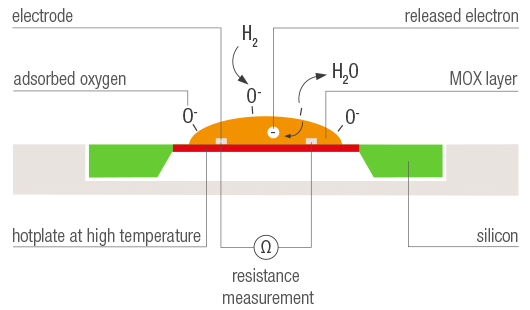
\includegraphics[width=.8\textwidth]{figures/moxGasSensor.png}
        \caption{MOX gas sensor technology~\cite{Sensirion}.}
        \label{fig:moxGasSensor}
    \end{figure}

    At operating temperature different gases react with oxygen atoms at the surface, contributing for the MOX layer's
    resistivity change, while at high temperatures the adsorbates are removed~\cite{labManual}.
    Gases such as VOCs (reducing gases) and $\mathrm{NO_x}$ (oxidizing gases) compounds can lower or increase the
    resistance of the MOX layer respectively~\cite{labManual}.
    Water molecules also play a role in the resistivity change of the MOX layer~\cite{labManual}.
    MOX gas sensors are highly sensitive, but their selectivity is poor~\cite{labManual}.

    BME688 is equipped with a Bosch Software Environmental Cluster BSEC algorithm~\cite{BME688} that can process the sensor data and convert
    it into meaningful information.
    BSEC is designed to process the sensor data, compensate for temperature and humidity influences, and
    provide real-time IAQ, temperature, humidity, and pressure information as well as the concentration
    of different gases~\cite{BME688}.
    To target different gas classes, the sensors' application-specific integrated circuit (ASIC) applies the heat profile
    shown in Figure~\ref{fig:heatProfile} and interprets the data using the BSEC algorithm.

    \begin{figure}[!h]
        \centering
        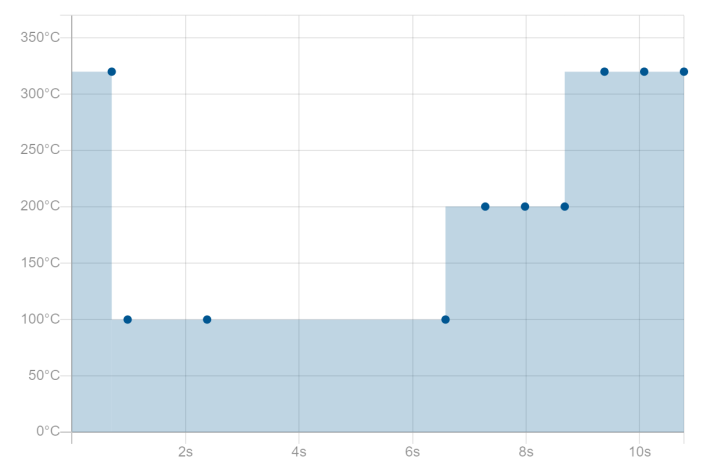
\includegraphics[width=.8\textwidth]{figures/heatProfile}
        \caption{Heat profile applied by BME688 and points where features are extracted~\cite{BME688}.}
        \label{fig:heatProfile}
    \end{figure}

    BSEC algorithm also calculates and indoor air quality index.
    The values vary from 0 to 500, where 0 is the best~\cite{BME688}.
    The classification of the values is given by Figure~\ref{fig:iaqTable}.

    \begin{figure}[!h]
        \centering
        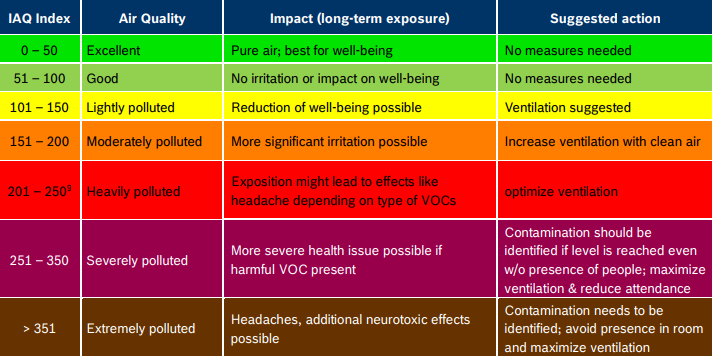
\includegraphics[width=.8\textwidth]{figures/iaqBme688}
        \caption{Indoor Air Quality (IAQ) index provided by BSEC~\cite{BME688}.}
        \label{fig:iaqTable}
    \end{figure}

    \section{Methods}\label{sec:methods}
    A battery-powered notebook was used to take all measurements from an Arduino Nicla Sense Board ME containing a BME688.
    It was connected to the computer via USB.
    The same notebook was used as a power supply for the board as well as a data logger.
    The board was programmed using the Arduino IDE 2.0.2 with the \texttt{Arduino\_BHY2} library version 1.0.6 (Bosch Sensortec).
    A small MATLAB application called \textit{SampleNicla} was developed to log the data.
    MATLAB was also used to process the data.
    The source code is available in \href{https://github.com/RafasLectures/sensorslab/blob/main/SampleNicla.mlapp}{GitHub}
    (\texttt{https://github.com/RafasLectures/sensorslab/})

    In a \SI{0.1}{\hertz} sampling rate (every \SI{10}{\second}), the Arduino program reads the gas
    virtual sensors \texttt{SENSOR\_ID\_GAS} and \texttt{SENSOR\_ID\_BSEC} from the BME688.
    The resolution of the gas sensor resistance measurement is typically 0.08\%~\cite{BME688}.

%    The sensor has a measurement range of 0-10,000 ppm for $\mathrm{CO_2}$, and 0-6,000 ppb for VOCs.
%    Its accuracy is ± (5\% of reading + 20 ppb) for VOCs and ± (5\% of reading + 50 ppm) for $\mathrm{CO_2}$.

    In Task~1 and 2, 55 to 75 measurements (550 \si{\second} to 750 \si{\second}) were taken while the sensor was exposed in each VOC source.
    Before exposing the sensor to the VOC source the program was running for at least 30 minutes, until it reached accuracy level 3.
    The chosen VOC sources were:

    \begin{enumerate}
        \item Coffee beans.
        \item A\c{c}a\'i powder
        \item Mate tea
    \end{enumerate}

    For each VOC source the sensor was placed inside the bag of it without touching the inside.
    Not the walls of the package, neither the content itself.
    The opening of the bag was reduced to try to have less influence of air going out of the bag.
    The recording of the measurements started outside the bag.
    After 10 measurements the sensor was placed inside, after 55 to 75 measurements it was removed from the bag
    and after the resistance was around the value it was initially before the measurements, the recording stopped.

    Between the measurements of each VOC source, the sensor was left running for at least 10 minutes and the accuracy level
    was 3 before it was place inside the next bag to measure the next VOC source.

    Task 3 was done in my one-room apartment.
    The sensor was placed on my working desk, but not touching any surface.
    There was a microphone stand, and the sensor was being held by its cable which was being held by the microphone stand.
    There was no air being blown into the sensor and no sources of heat close to it.

    \section{Results and Discussion}\label{sec:results-and-discussion}

    \subsection*{Task 1, 2}

    The first and second task are intended to verify the resistance of the gas sensor as well as the BSEC algorithm to
    calculate the VOC and $\mathrm{CO_2}$.
    The Nicla Sense ME Board was placed inside three different VOC sources as described in~\nameref{sec:methods}.
    Figure~\ref{fig:vocSourceExposure}, shows the resistance of the sensor as well as the calculated VOC and $\mathrm{CO_2}$ for
    the different VOC sources.

    \begin{figure}[h]
        \centering
        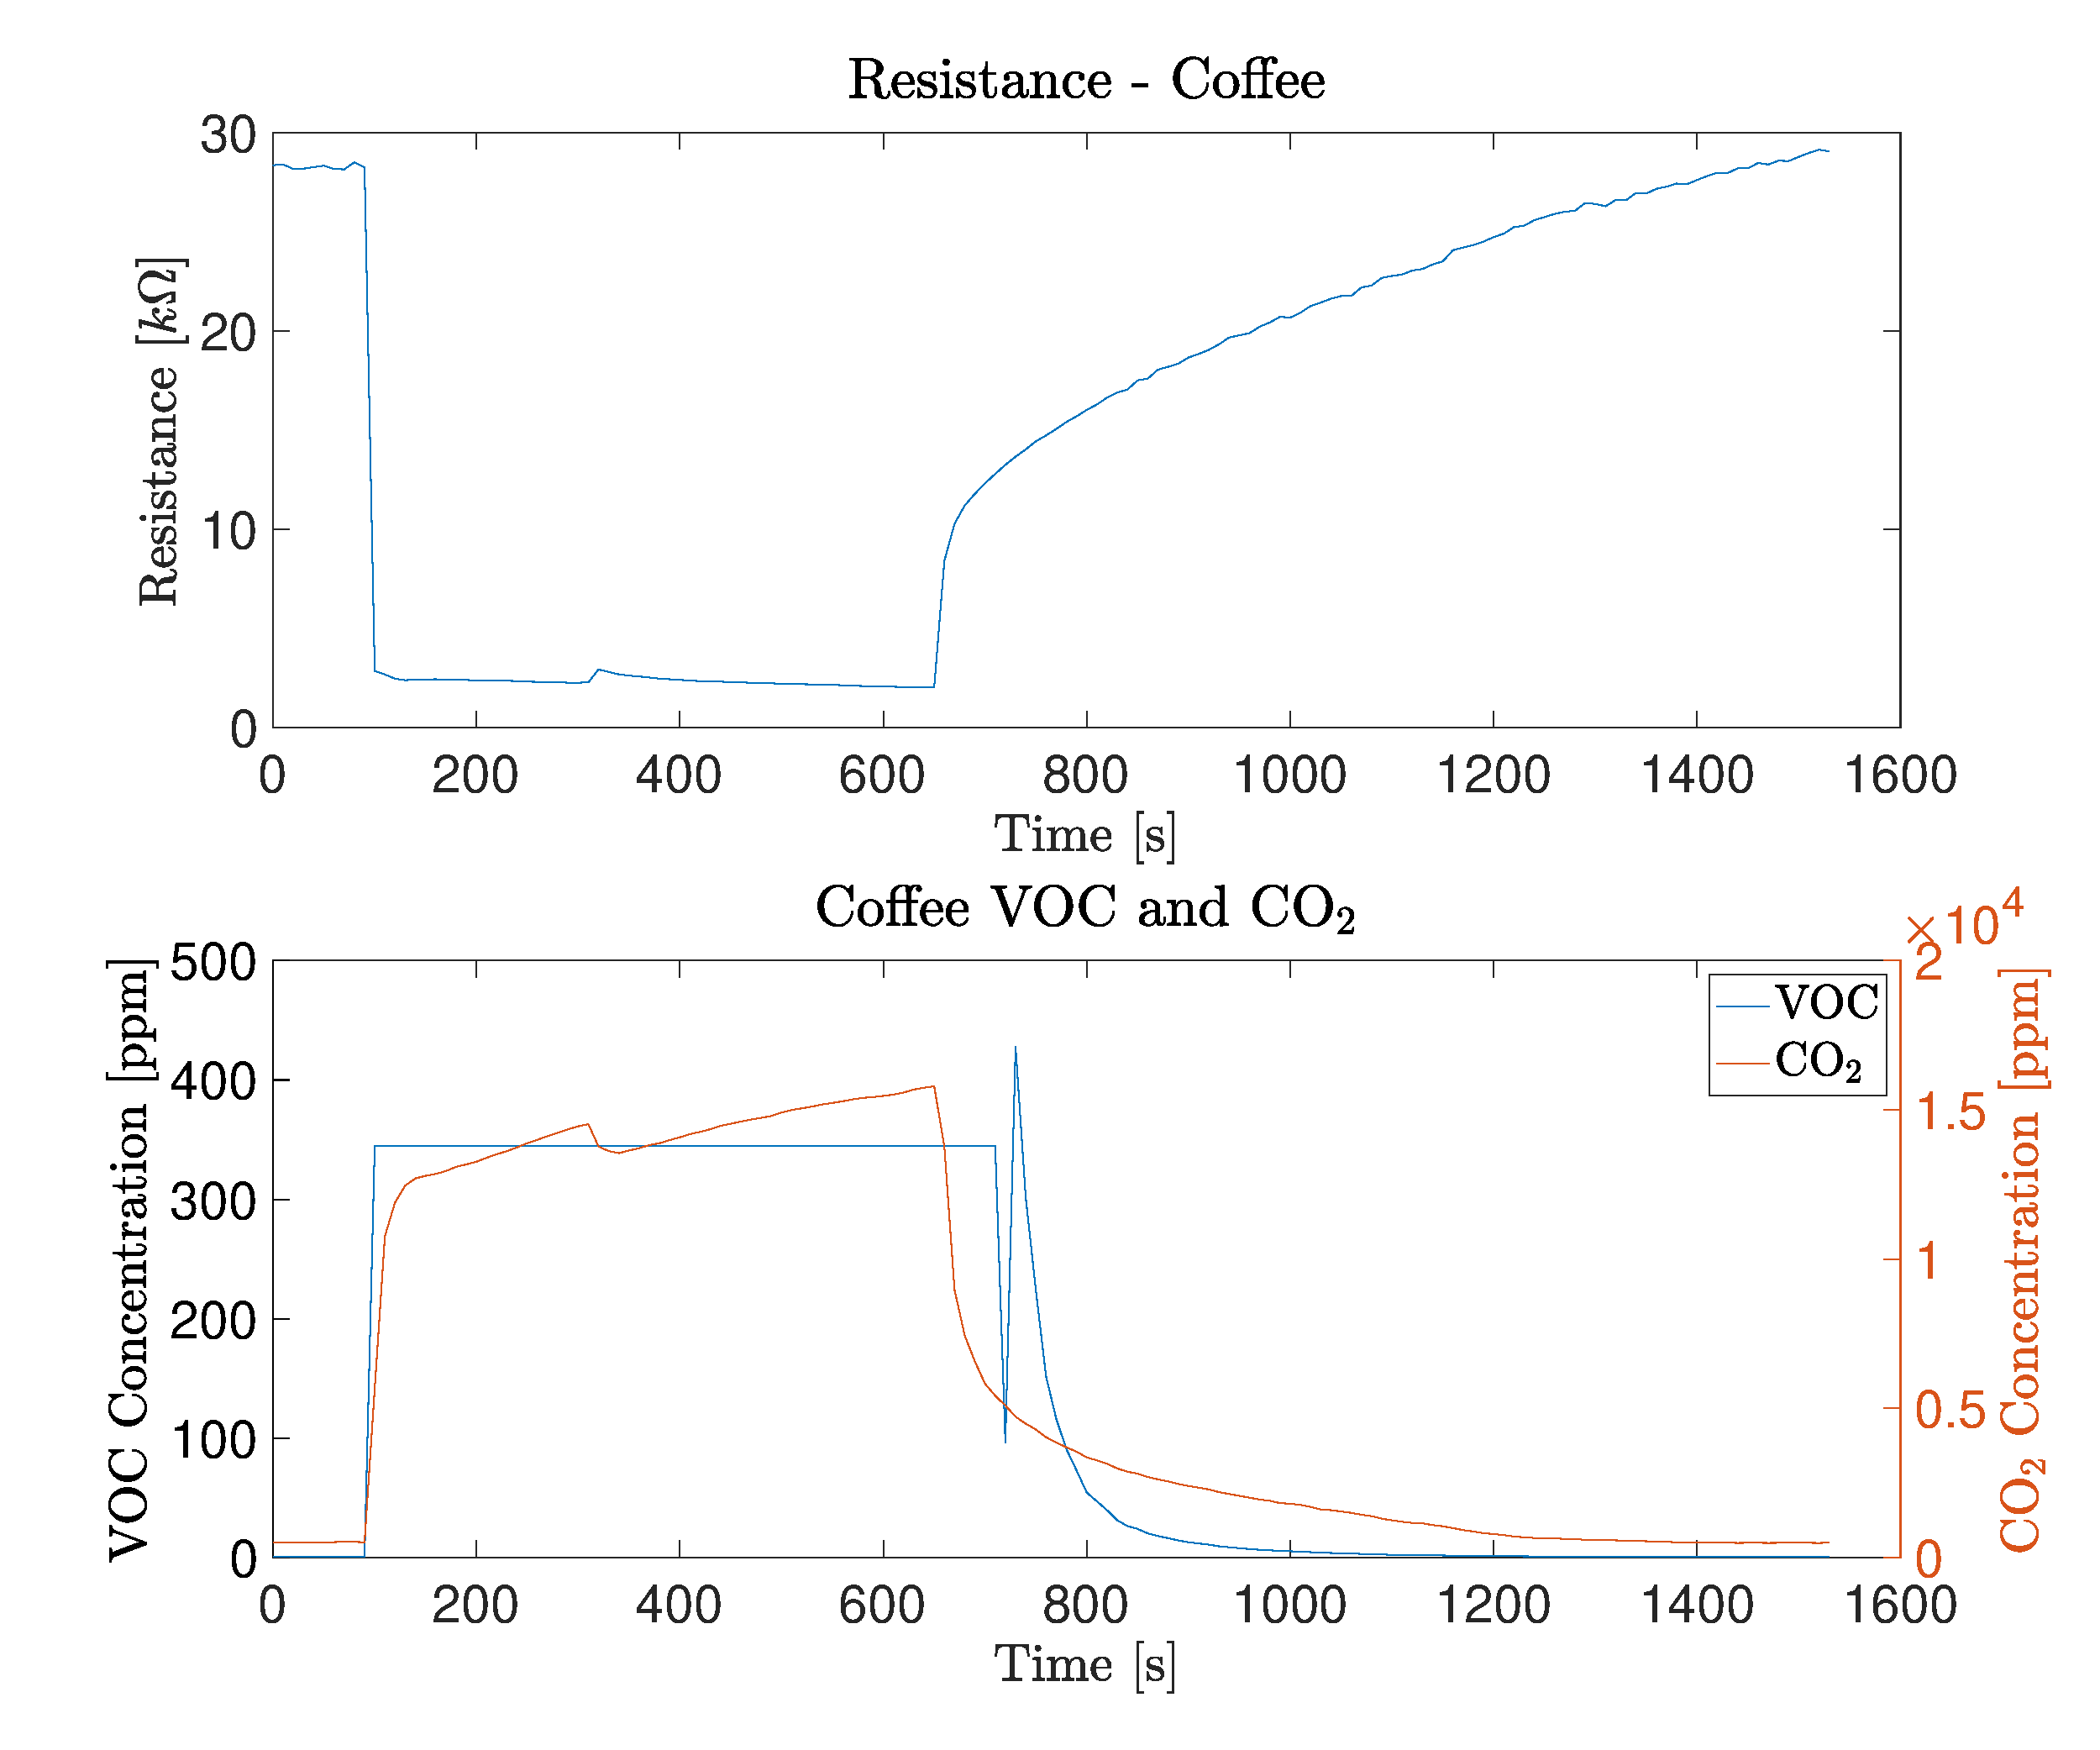
\includegraphics[width=.45\textwidth]{plots/plotCoffee}
        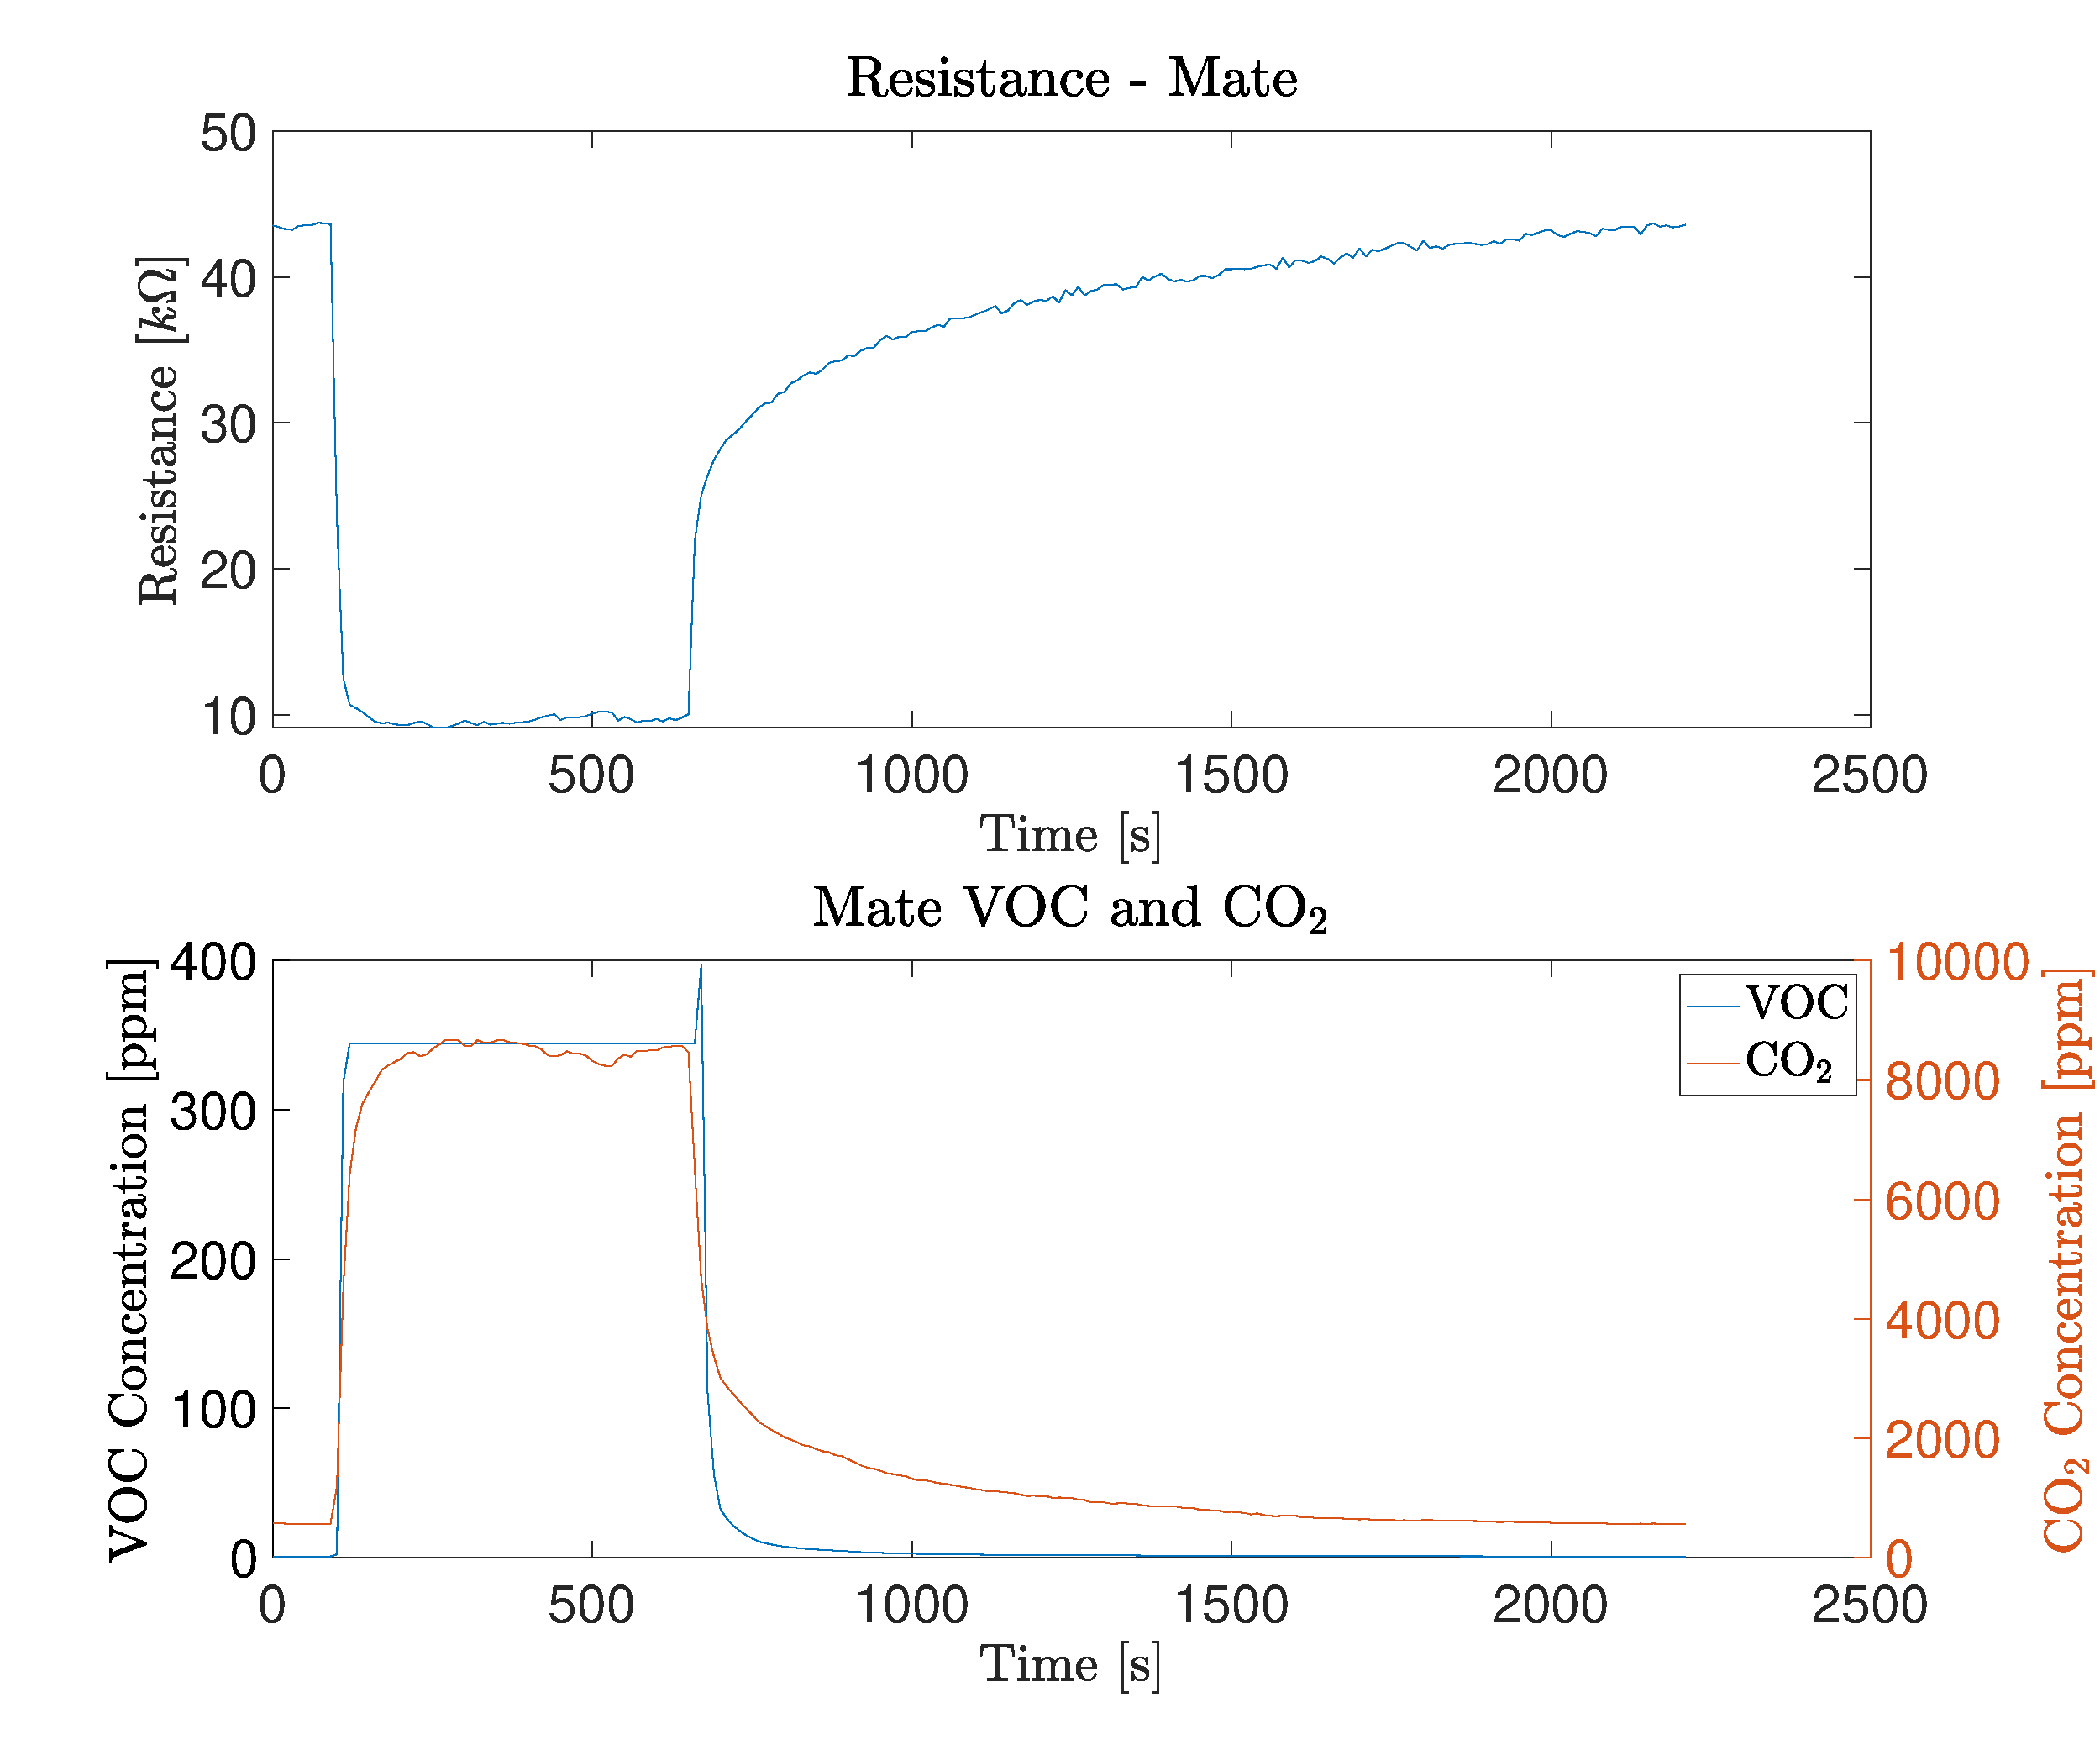
\includegraphics[width=.45\textwidth]{plots/plotMate}
        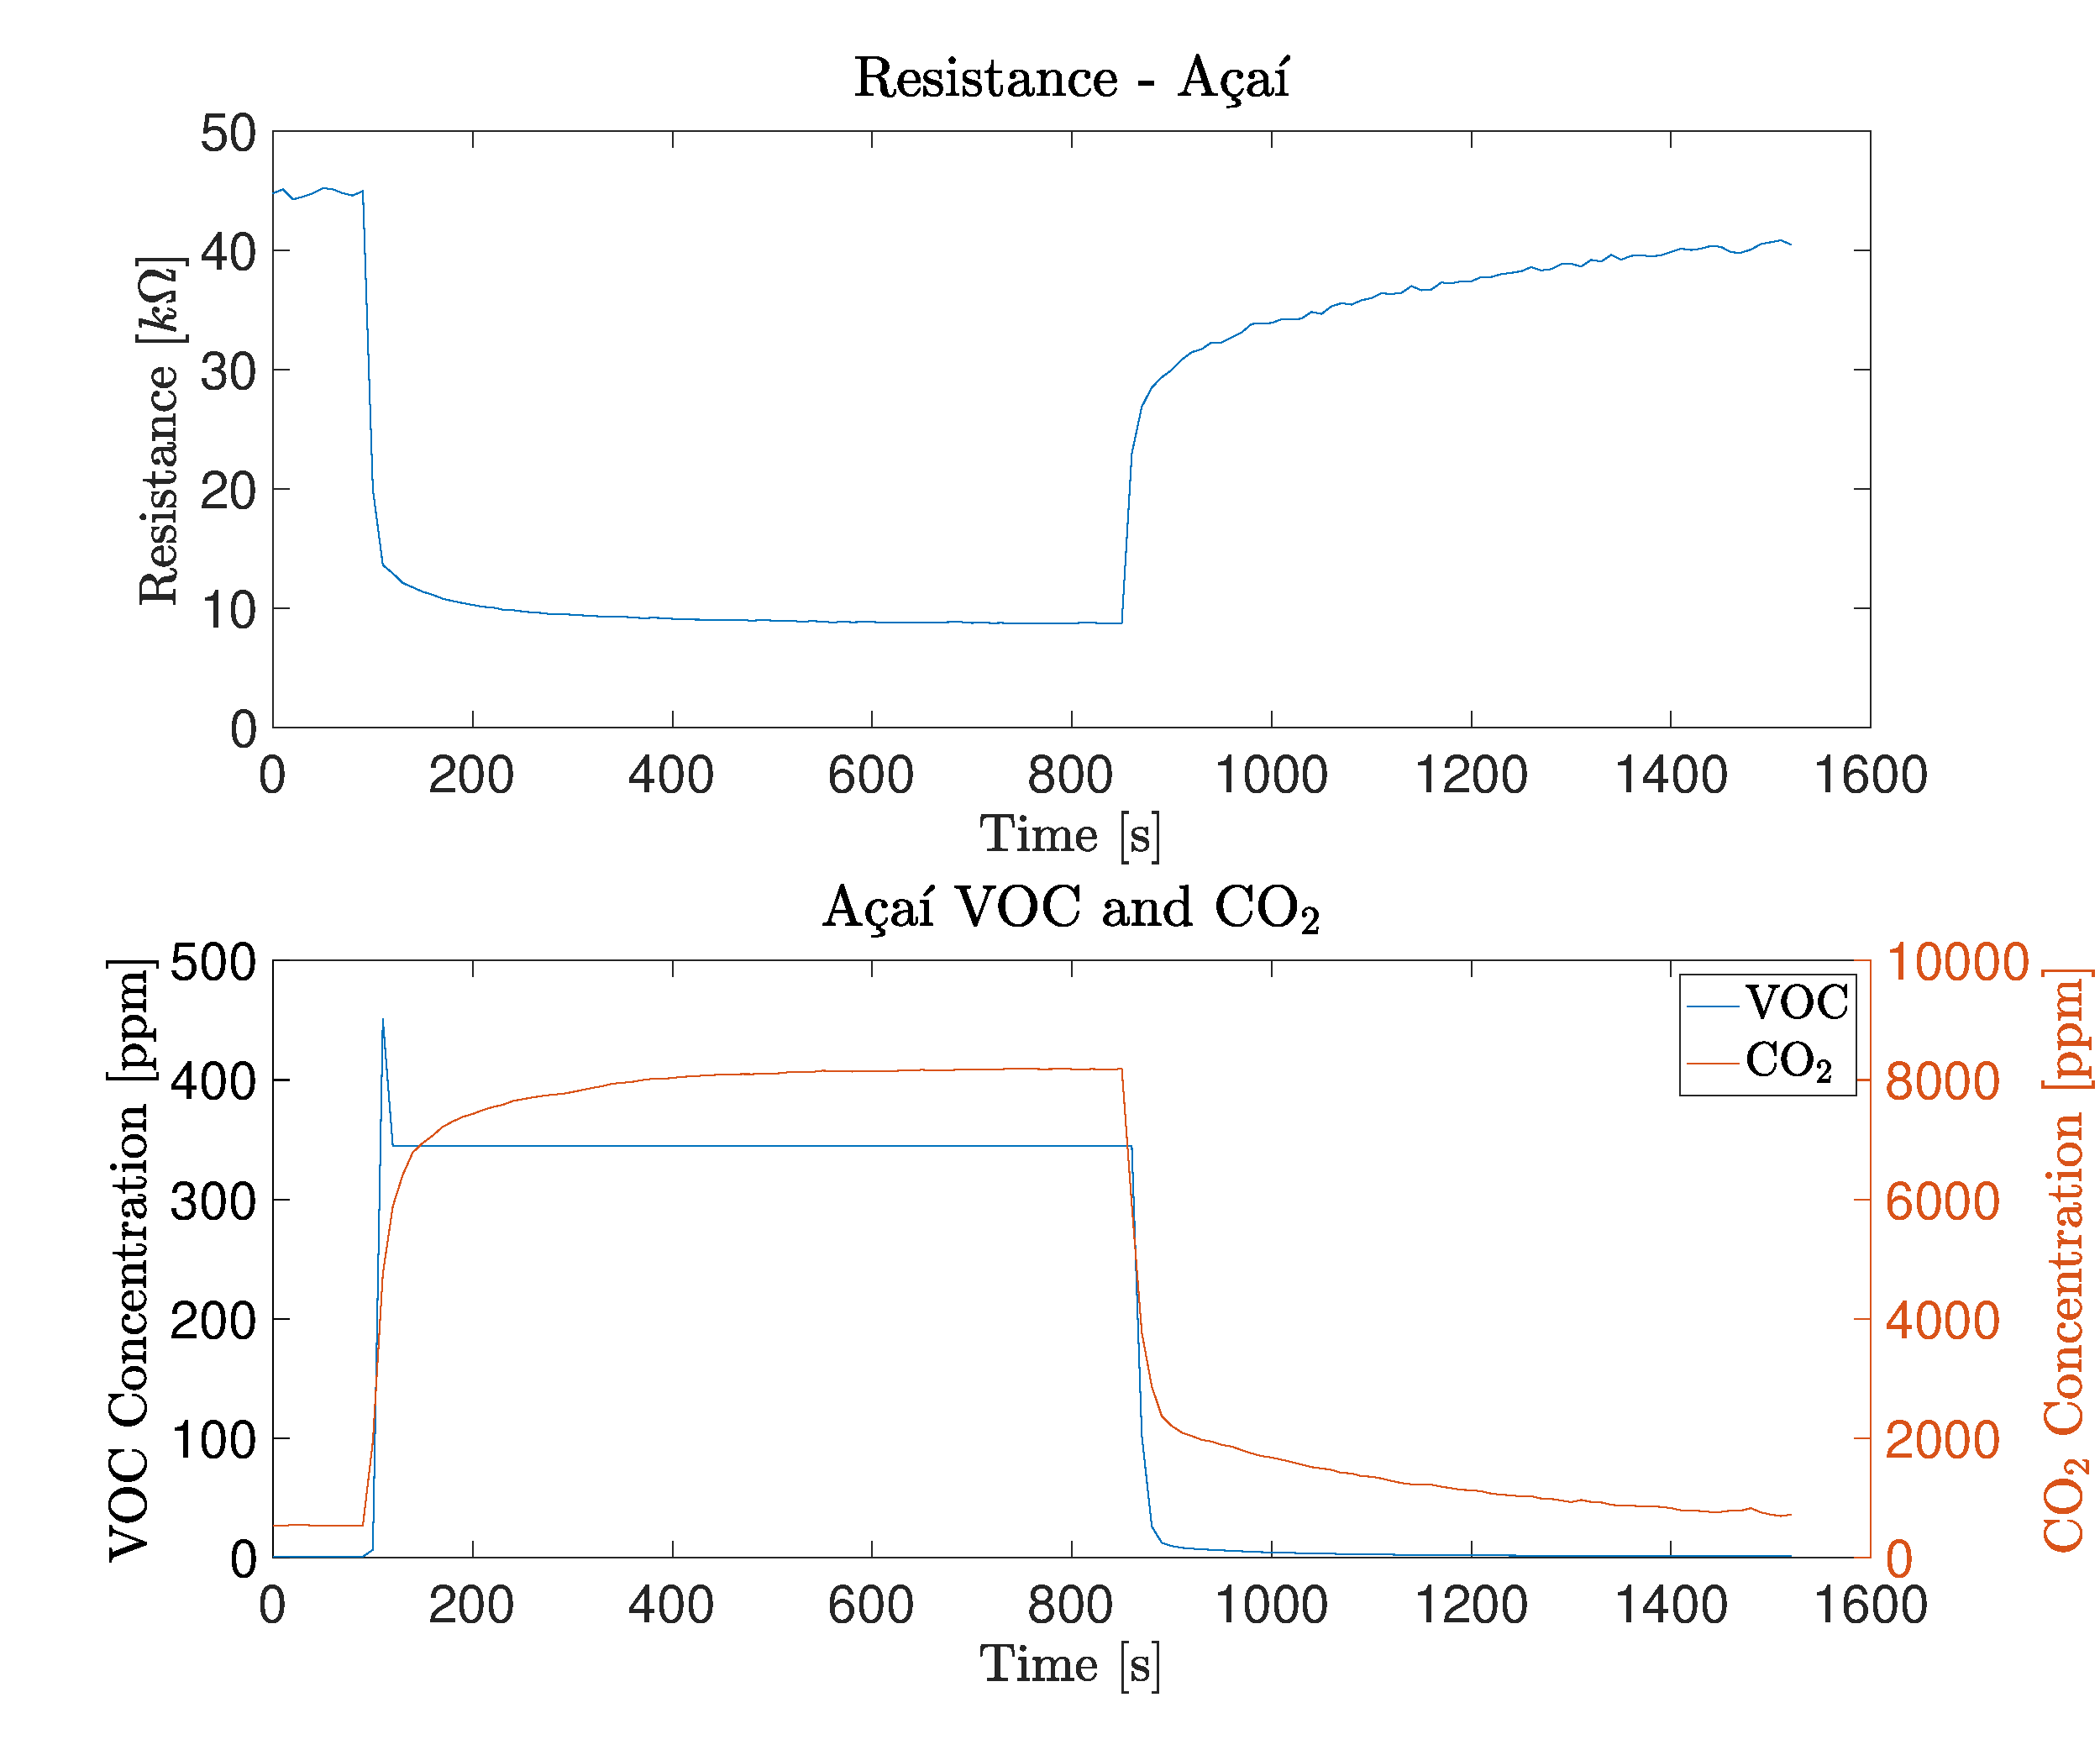
\includegraphics[width=.45\textwidth]{plots/plotAcai}
        \caption{Plots of the resistance and calculation of VOC and $\mathrm{CO_2}$ of the different VOC sources.}
        \label{fig:vocSourceExposure}
    \end{figure}

    The resistance of the sensor, when exposed to the VOC sources is not constant.
    For the a\c{c}a\'i and the coffee it kept getting smaller as the exposure time increased.
    For the coffee it dropped 400\si{\ohm} during the exposure time.
    For the a\c{c}a\'i it dropped almost 1\si{\kilo\ohm}.
    In the mate measurement it oscillated more.
    The reason could be that the bag could not be very well closed as for the other two measurements.

    Tables~\ref{tab:resistance} and~\ref{tab:concentrations} summarize the results.

    \begin{table}[!ht]
        \centering
        \begin{tabular}{cS[table-format=1.3]cS[table-format=1.3]cS[table-format=1.3]}
            \hline \vspace{-1em} \\
            {VOC source} & {Average Resistance}       & {Resistance recovery}  \\
                         & {on exposure in \si{\ohm}} & {time in \si{\second}} \\ \hline
            Coffee Beans & 2200                       & 880                    \\
            A\c{c}a\'i   & 9000                       & 670                    \\
            Mate         & 9500                       & 1560                   \\
        \end{tabular}
        \caption{Summary of the resistance for different VOC sources.}
        \label{tab:resistance}
    \end{table}

     \begin{table}[!ht]
         \centering
         \begin{tabular}{cS[table-format=1.3]cS[table-format=1.3]cS[table-format=1.3]cS[table-format=1.3]}
             \hline \vspace{-1em} \\
             {VOC source} & {VOC concentration} & {$\mathrm{CO_2}$ concentration}   & {VOC recovery}         & {$\mathrm{CO_2}$ recovery} \\
                          & {in ppm}            & {in ppm}                          & {time in \si{\second}} & {time in \si{\second}}     \\ \hline
             Coffee Beans & 344.64              & 14200                             &  730                   &  750                       \\
             A\c{c}a\'i   & 344.64              & 8100                              &  670                   &  670                       \\
             Mate         & 344.64              & 8400                              &  1540                  &  1540                      \\
         \end{tabular}
         \caption{Summary of the concentrations for different VOC sources.}
         \label{tab:concentrations}
     \end{table}



    \subsection*{Task 3}
    In task 3 the same information from task 1 and 2 were measured, but also the IAQ, temperature and humidity.
    The measurements were taken for 24h every 10 seconds.

    The results are shown in the Figures~\ref{fig:co2IaqAndVoc} and˜\ref{fig:tempHum}.

    \begin{figure}[!ht]
        \centering
        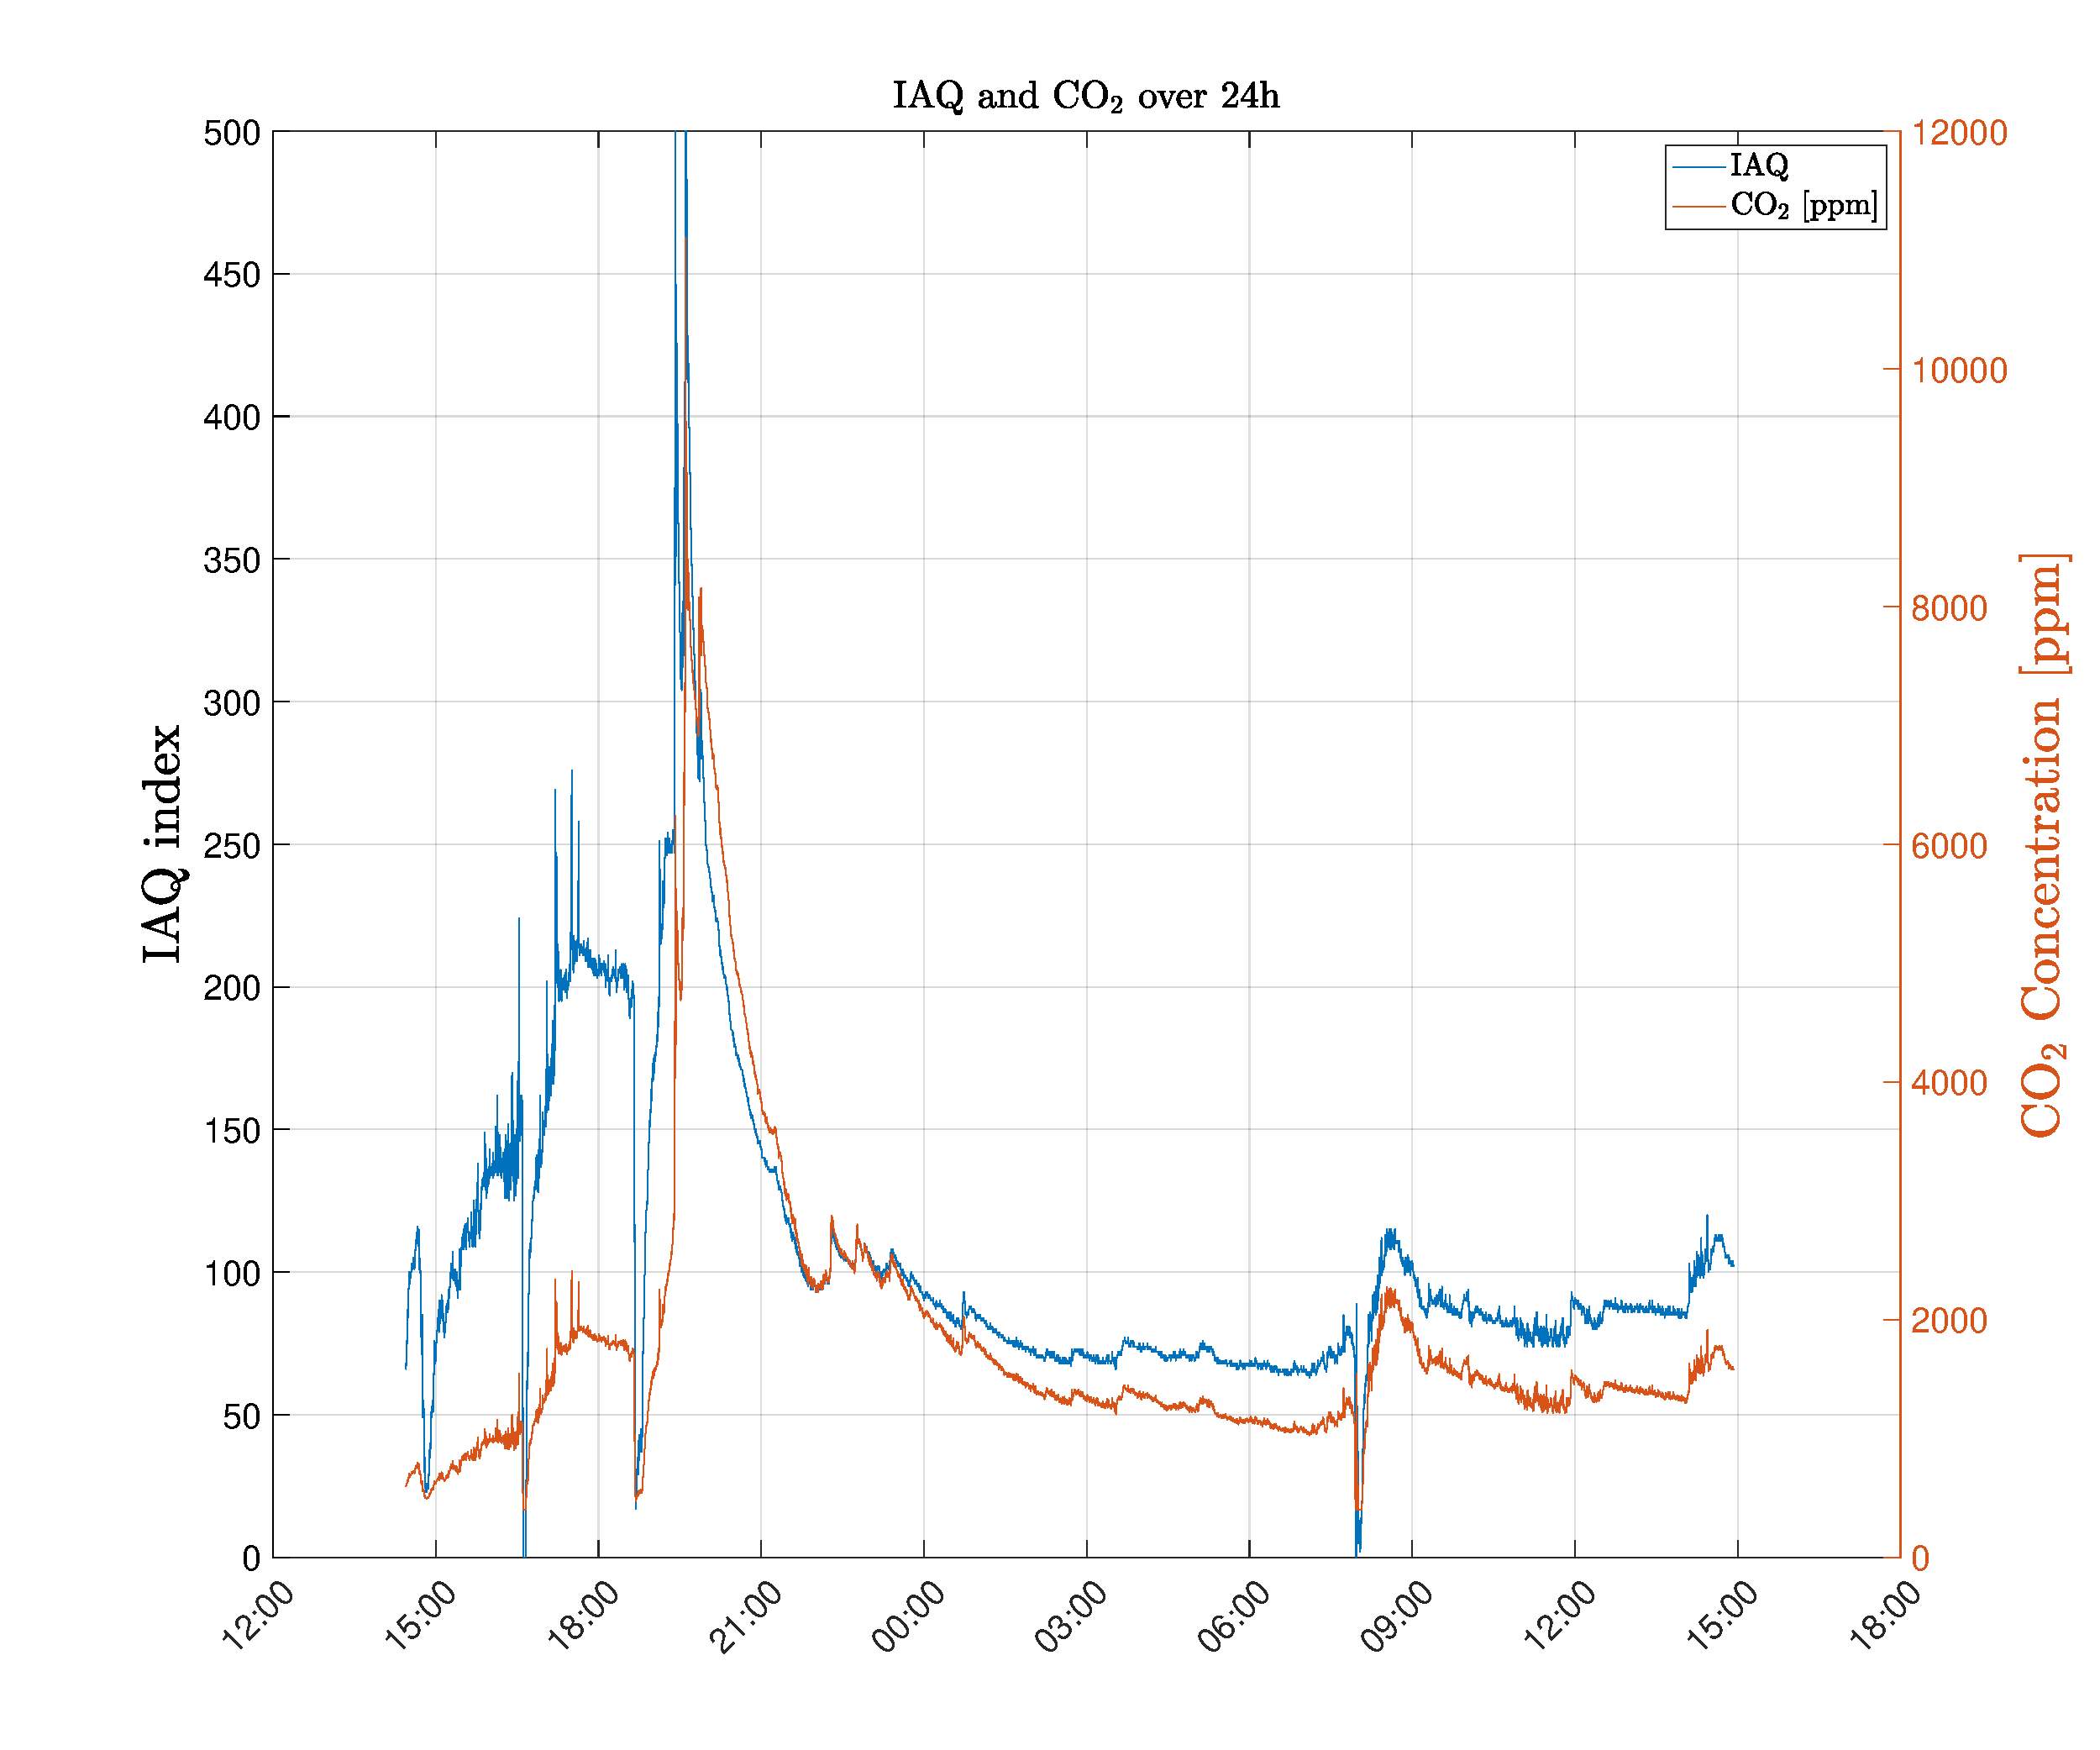
\includegraphics[width=.8\textwidth]{plots/plotCO2IAQ}
        \caption{$\mathrm{CO_2}$ and IAQ over 24h.}
        \label{fig:co2IaqAndVoc}
    \end{figure}

    \begin{figure}[!ht]
        \centering
        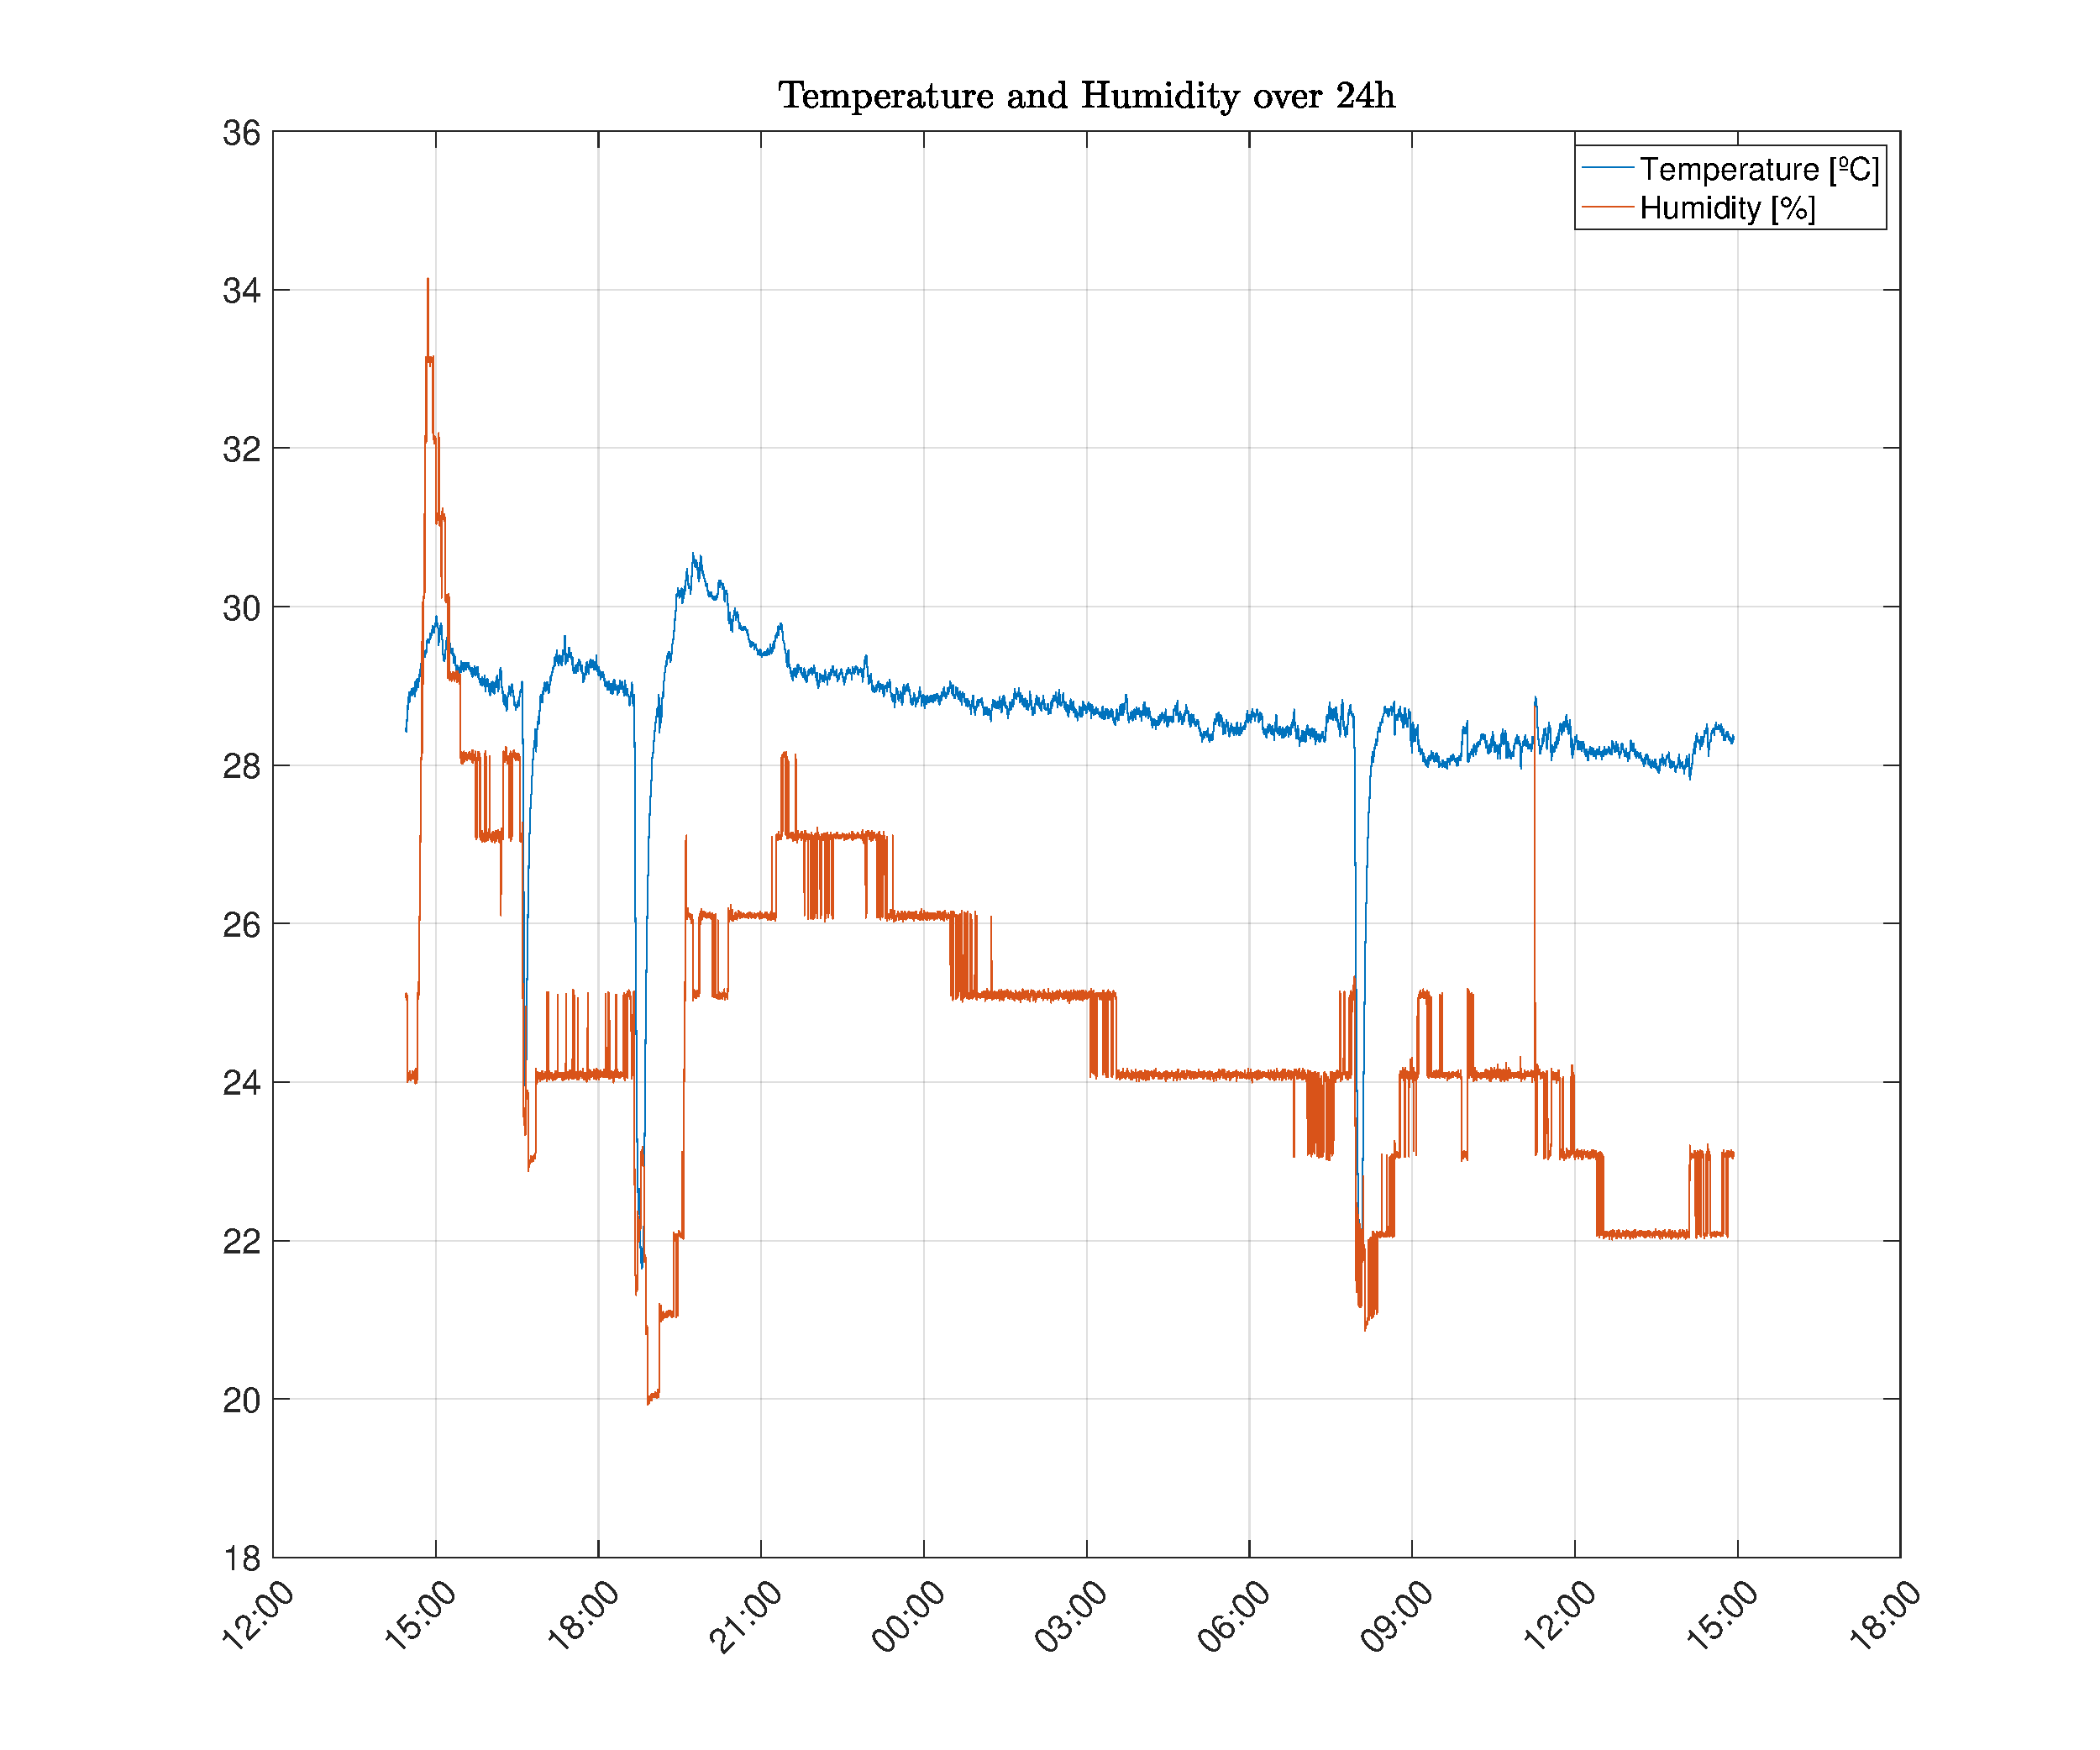
\includegraphics[width=.8\textwidth]{plots/plotTempHum}
        \caption{Temperature and humidity over 24h.}
        \label{fig:tempHum}
    \end{figure}

%    \begin{figure}[!ht]
%        \centering
%        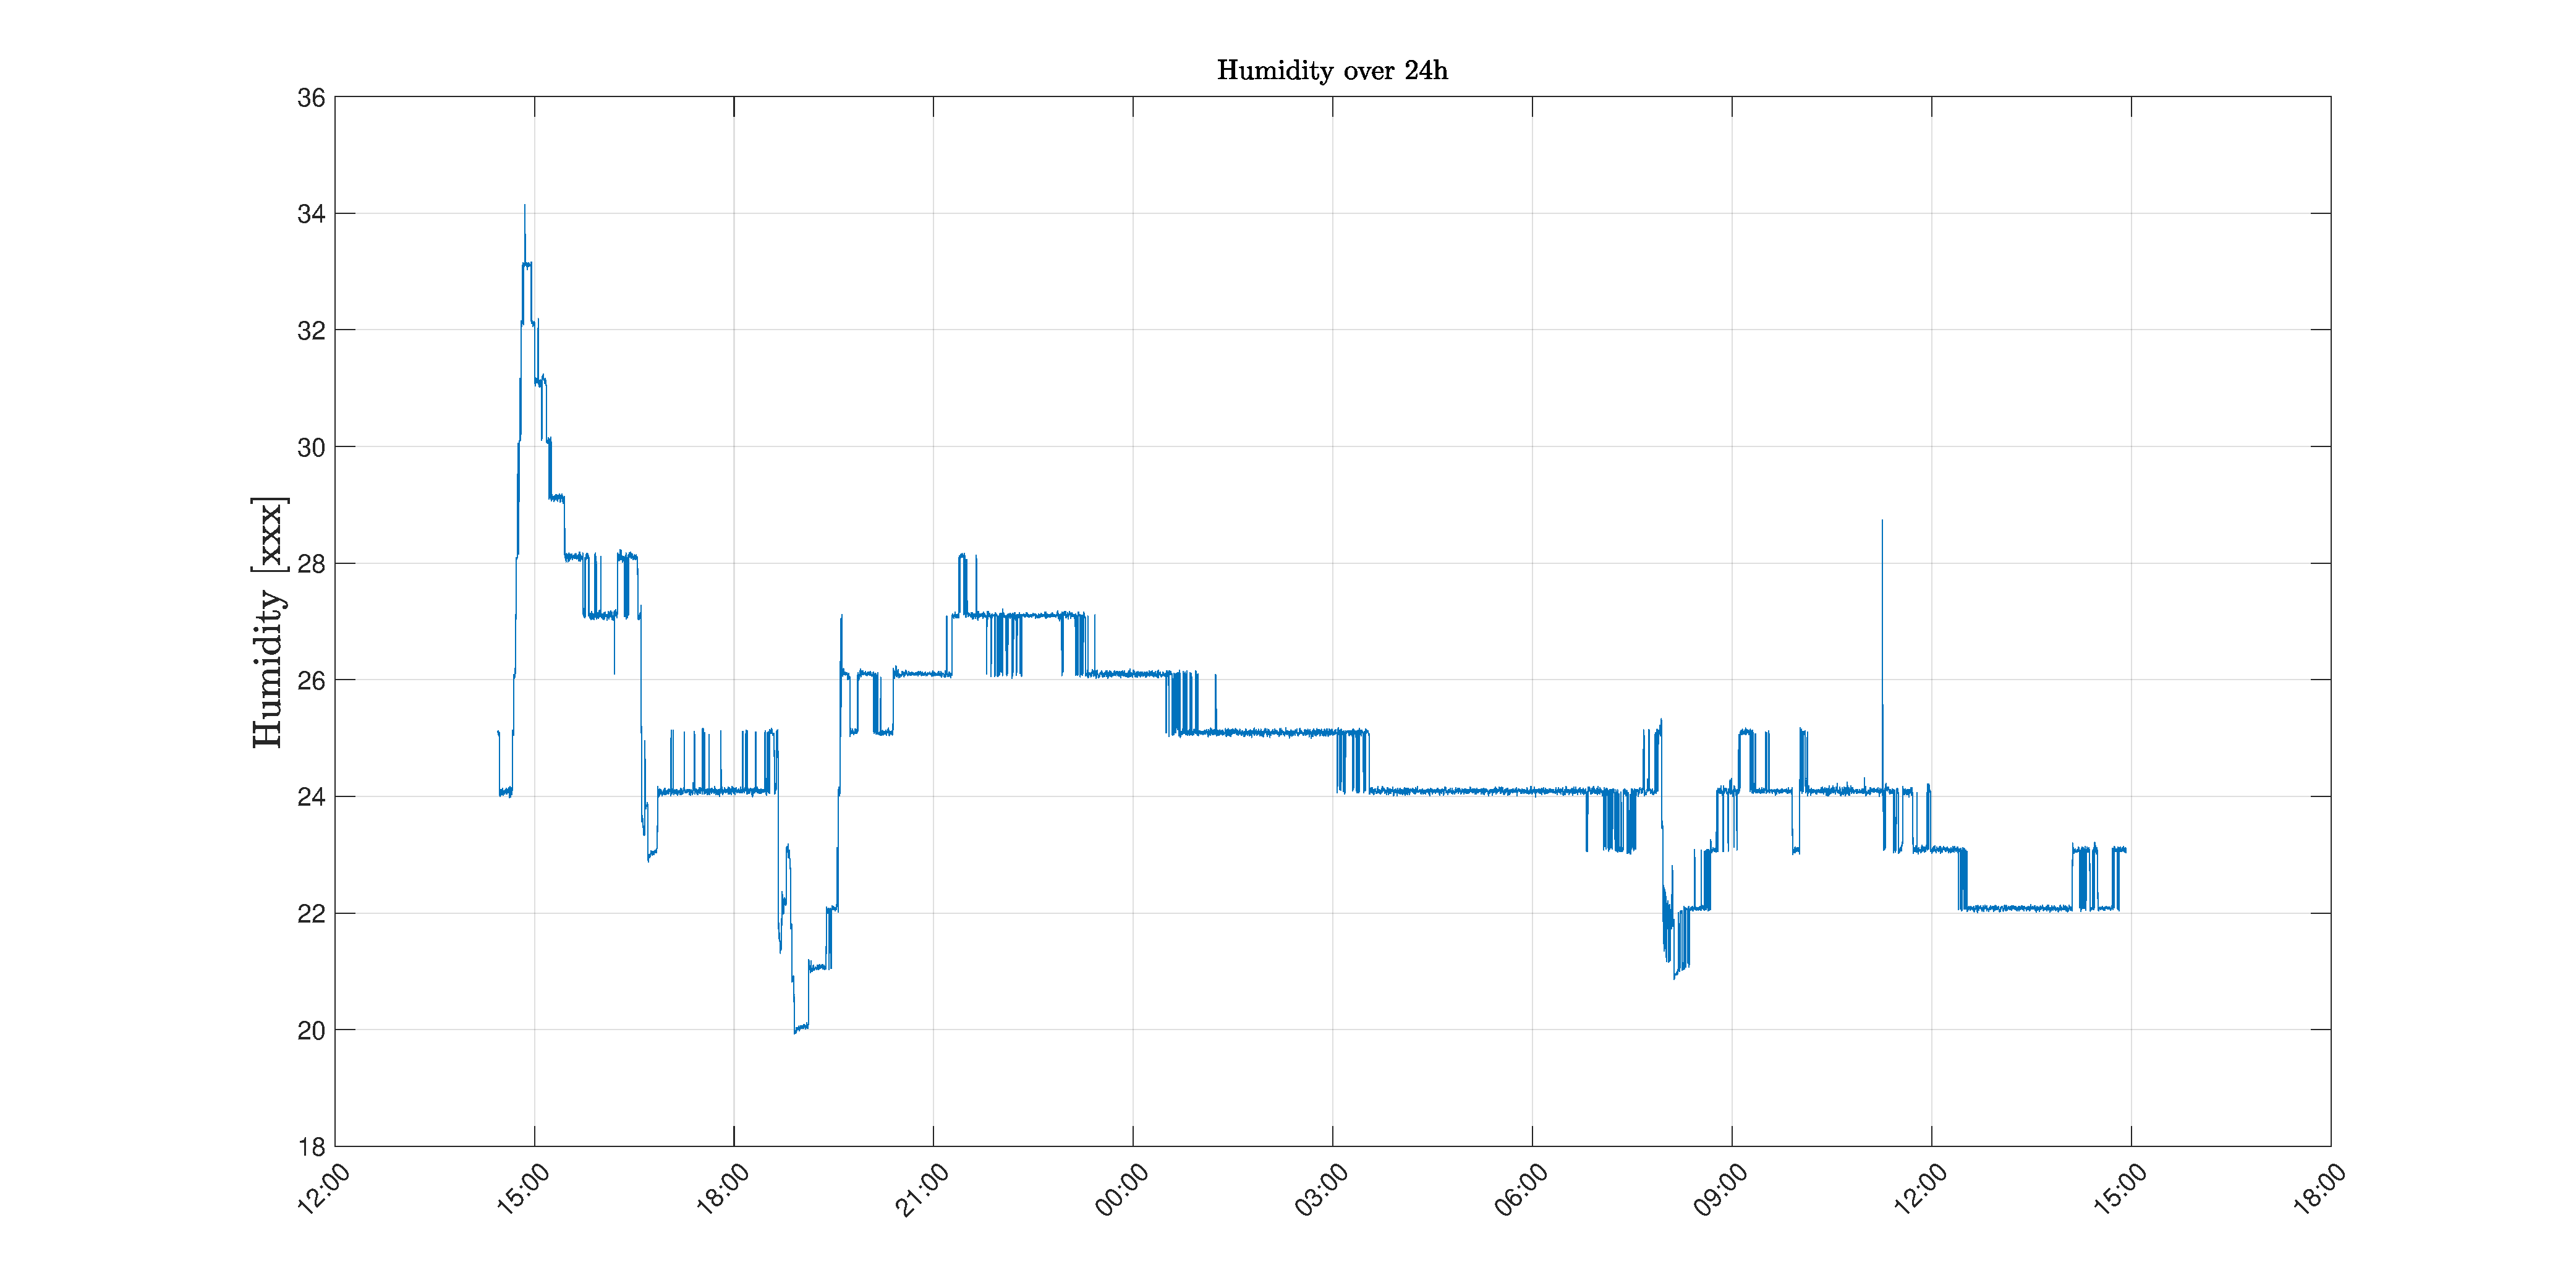
\includegraphics[width=.8\textwidth]{plots/plothum_idx}
%        \caption{Indoor Air Quality (IAQ) index provided by BSEC~\cite{BME688}.}
%        \label{fig:iaqTable}
%    \end{figure}
%
%
%    \begin{figure}[!ht]
%        \centering
%        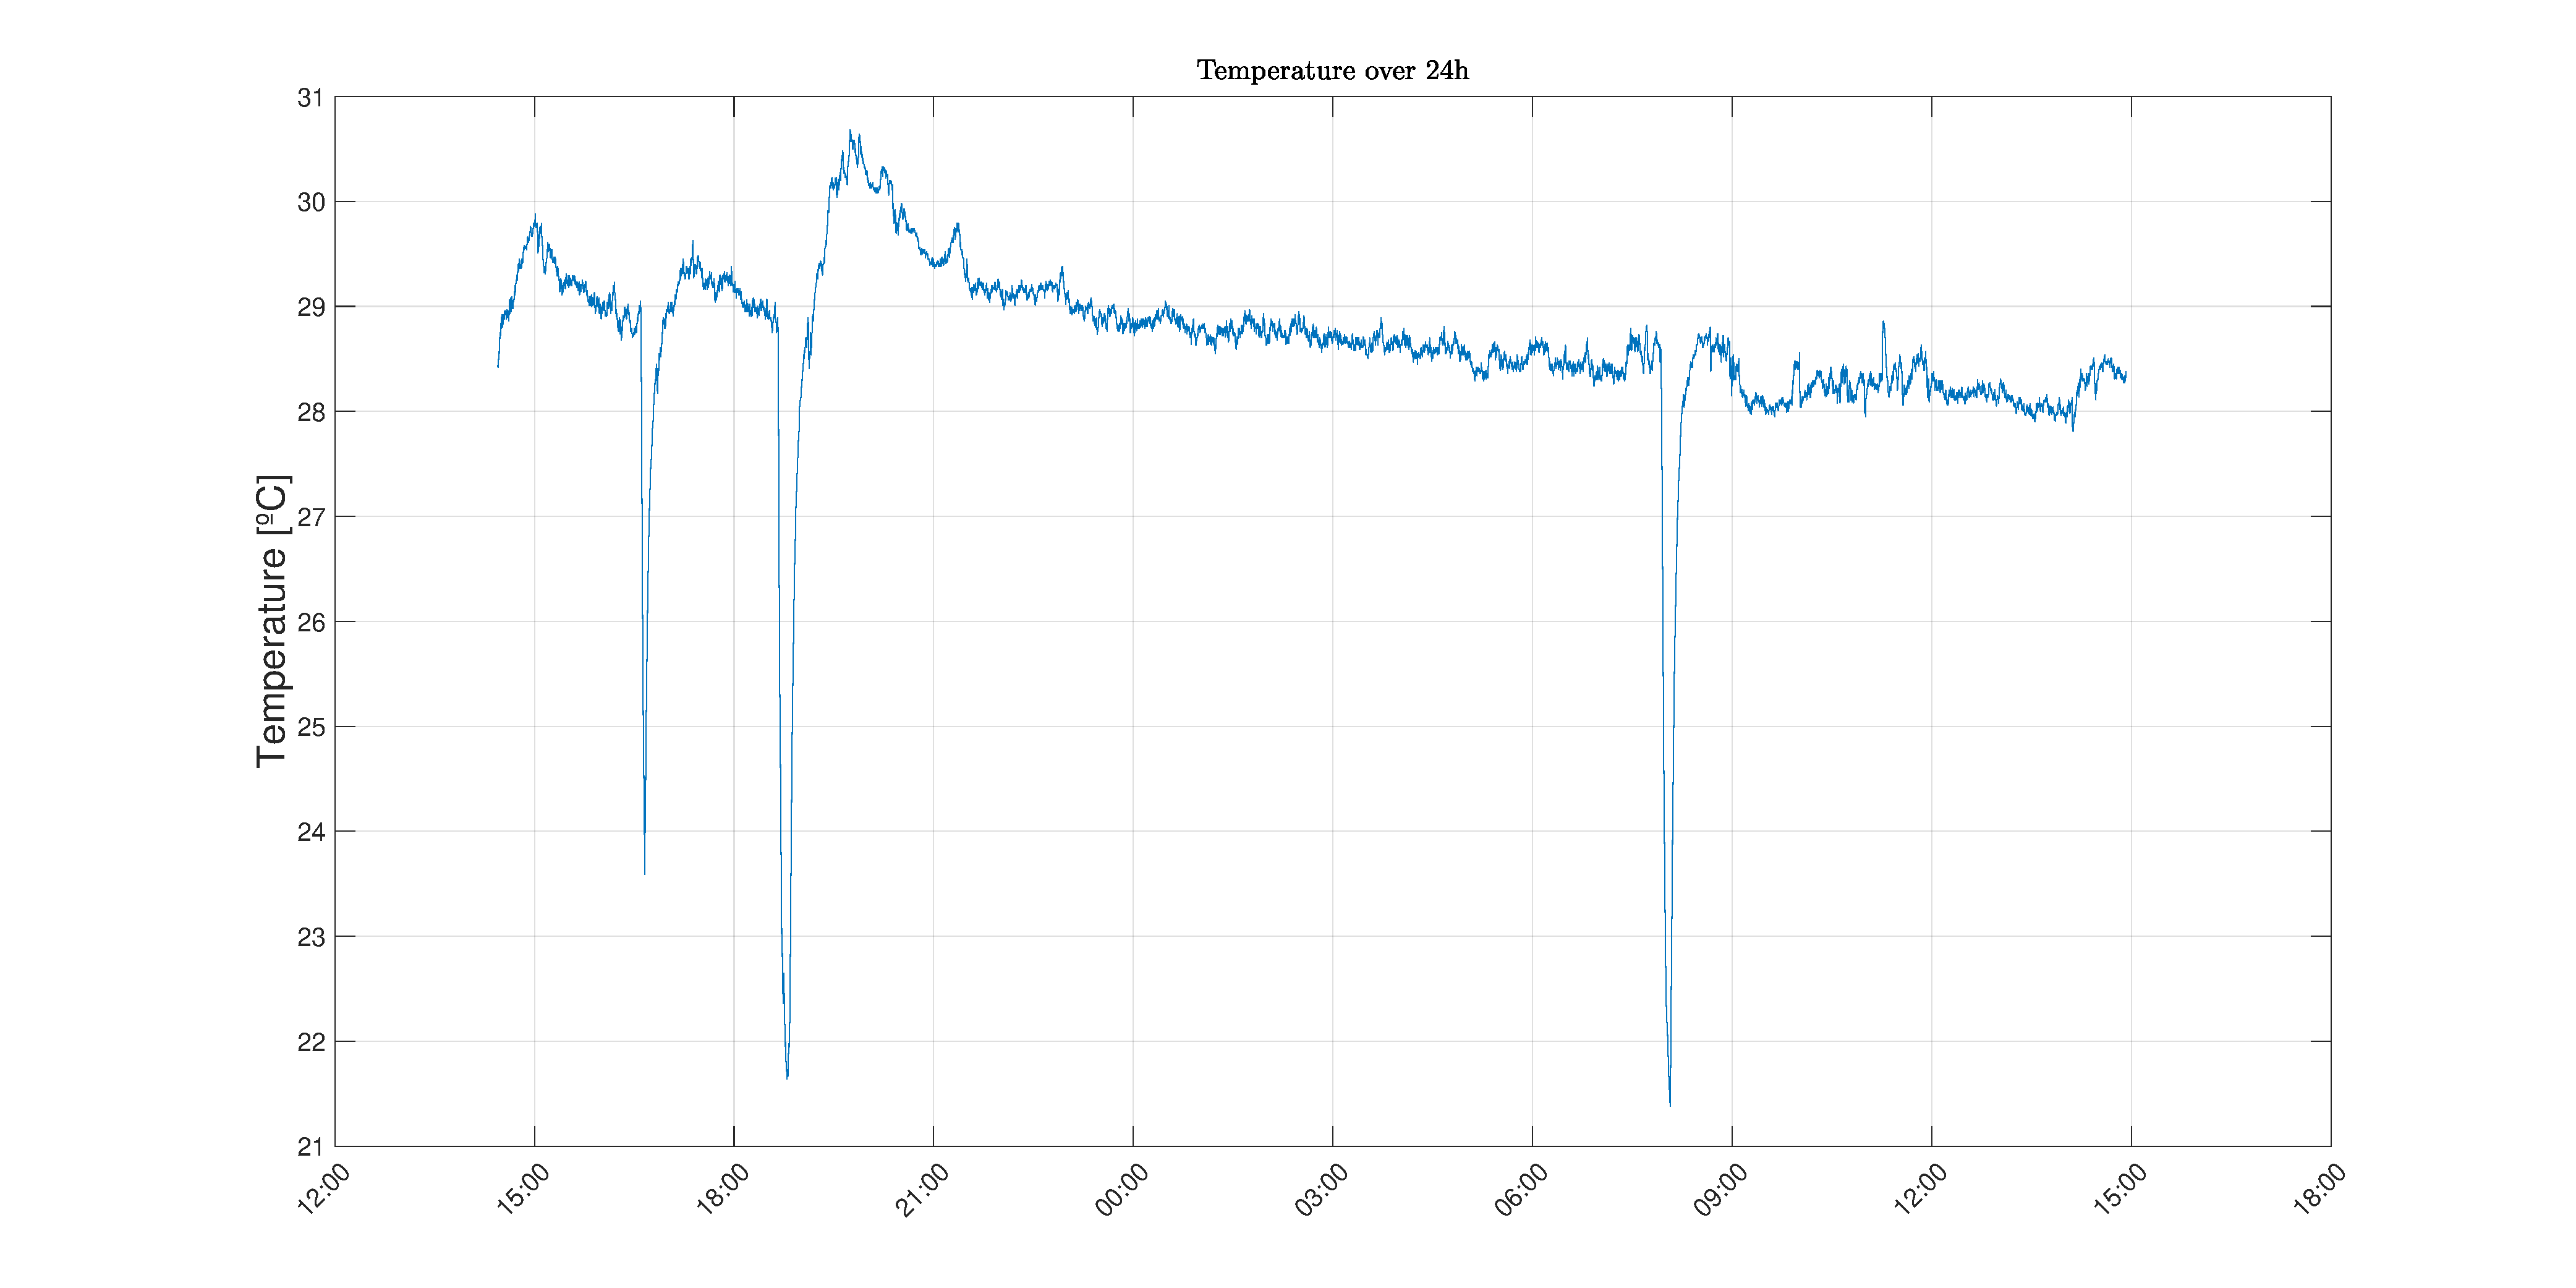
\includegraphics[width=.8\textwidth]{plots/plottemp_24h}
%        \caption{Indoor Air Quality (IAQ) index provided by BSEC~\cite{BME688}.}
%        \label{fig:iaqTable}
%    \end{figure}
%
%    \begin{figure}[!ht]
%        \centering
%        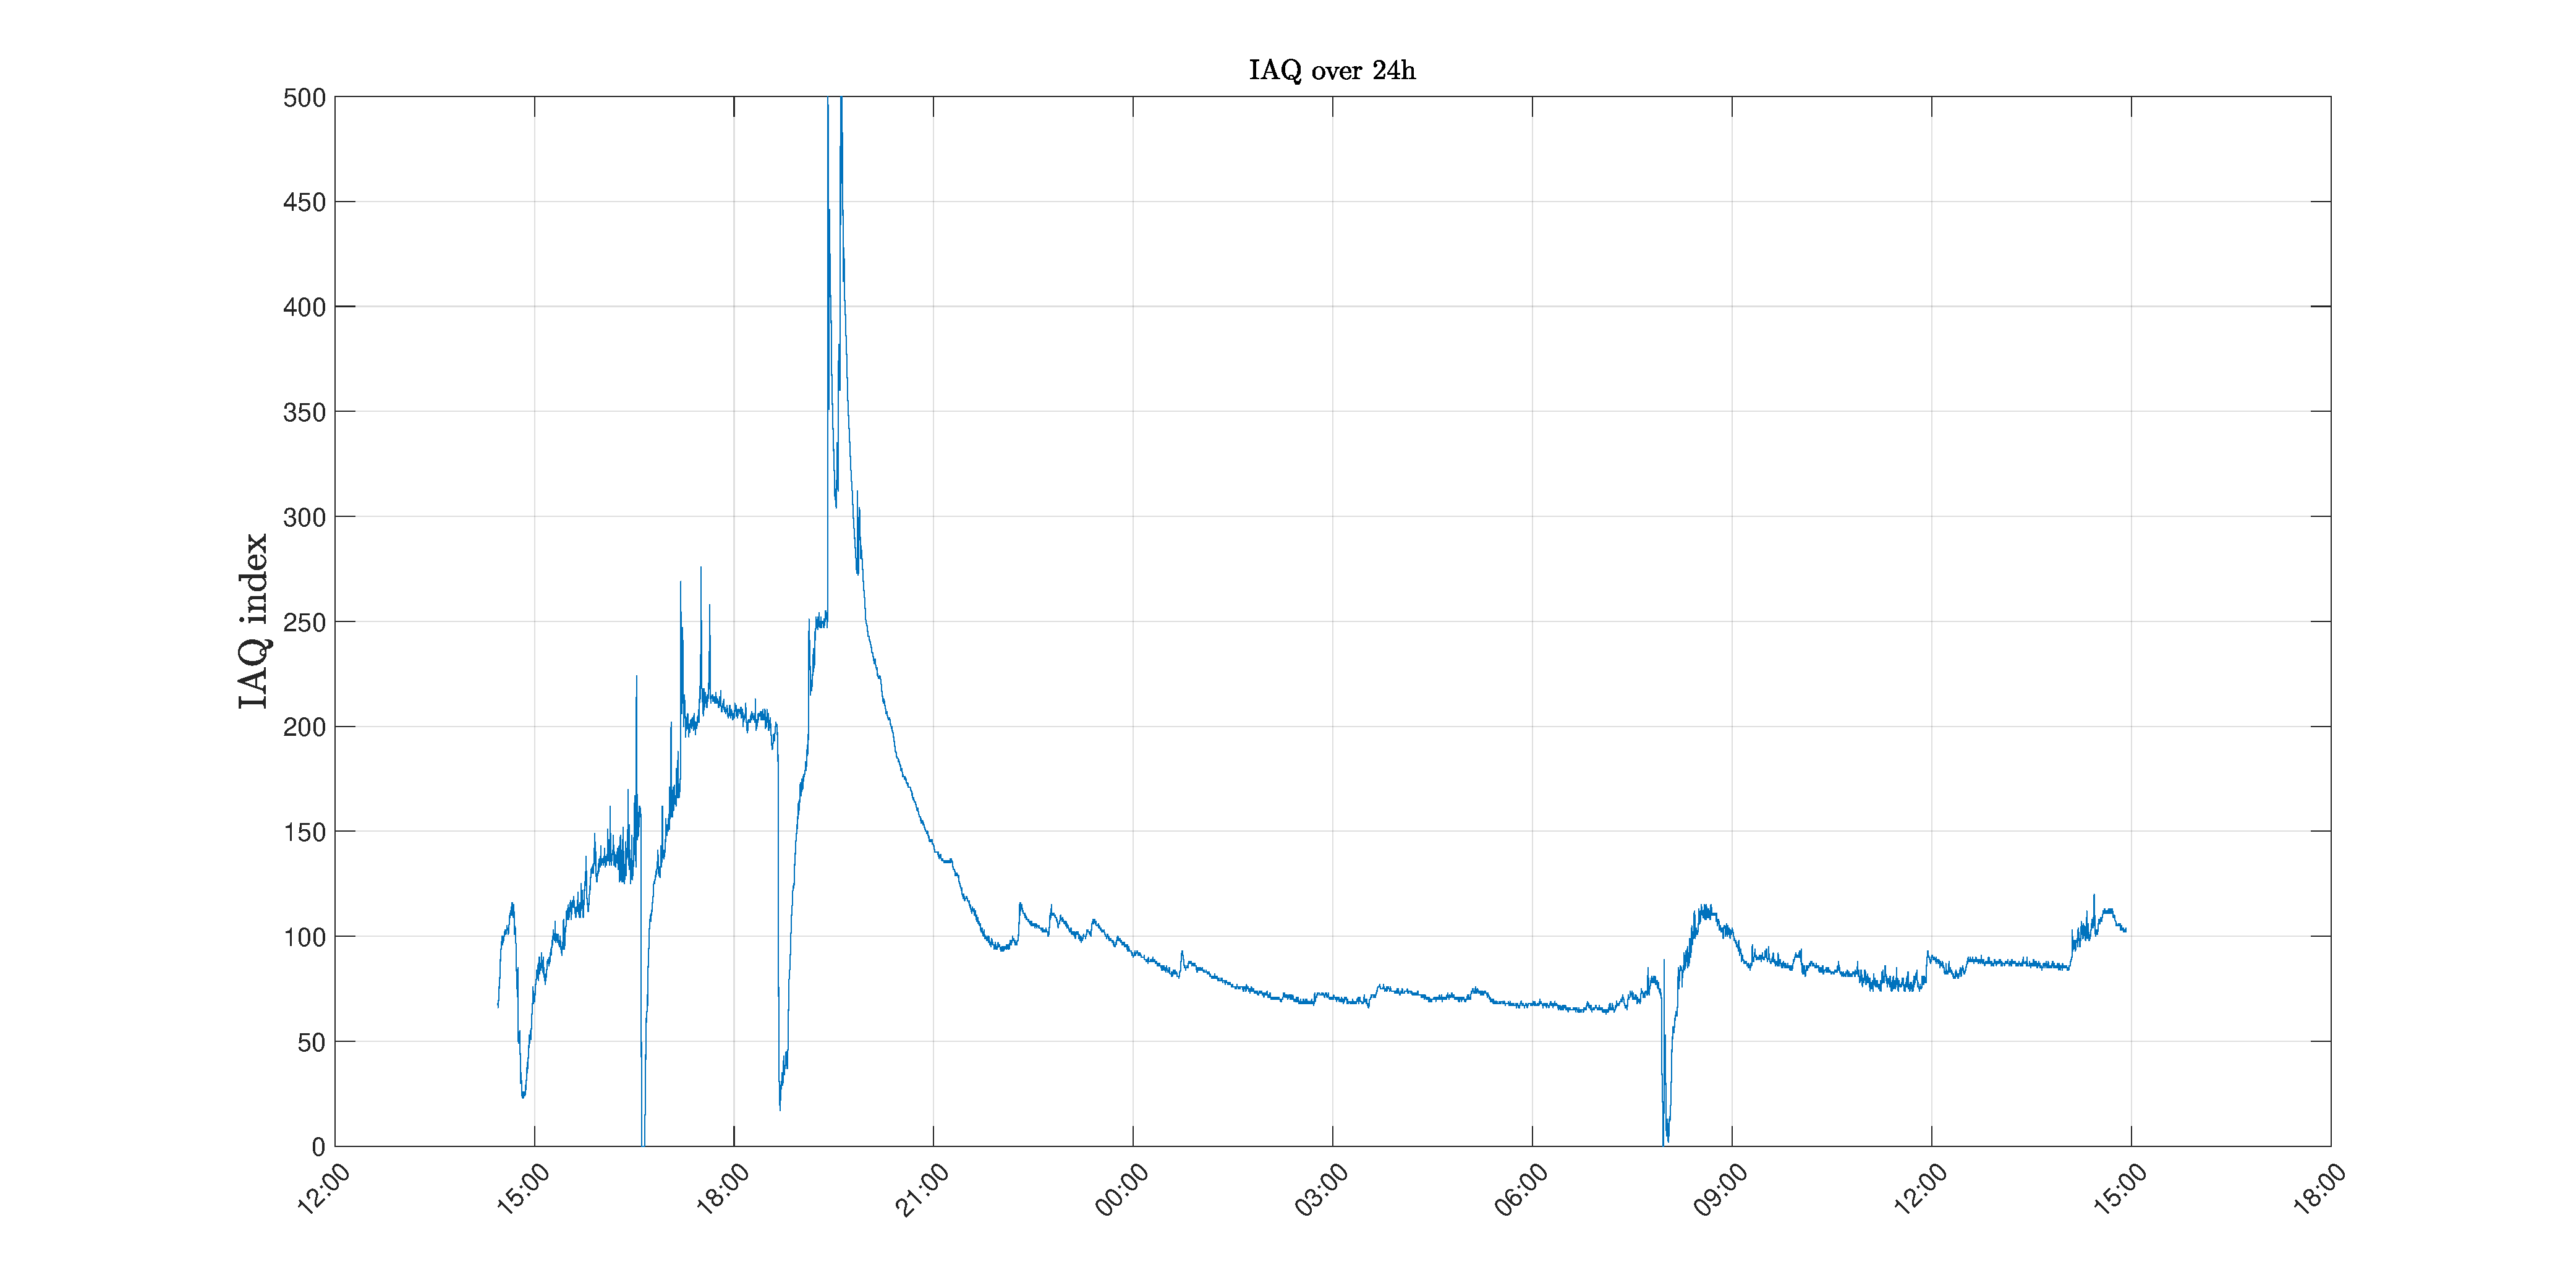
\includegraphics[width=.8\textwidth]{plots/plotiaq_idx}
%        \caption{Indoor Air Quality (IAQ) index provided by BSEC~\cite{BME688}.}
%        \label{fig:iaqTable}
%    \end{figure}

    Looking at Figure~\ref{fig:tempHum} one sees that the temperature was between 28 and 30 degrees, but it didn't feel so warm.
    I had a pullover all the time while home.
    Maybe due to where the sensor is located in the board, could have shifted the temperature.

    Although the temperature in general seems to have an offset, we can notice that there is three main temperature drops.
    At 16:40, 18:40 and 8:00.
    At those times I did air circulation by opening my window.
    We see that this three events are also visible in the humidity, IAQ and $\mathrm{CO_2}$ concentrations.

    The measurements started at 14:30.
    At 14:40 I started to cook some pasta and since it is a one-room apartment, the kitchen is in the same room as where the
    sensor was, and we can notice that the humidity increased 10\% around that time.

    From roughly 19:00 to 20:00 there is a peak in $\mathrm{CO_2}$ concentration and in the IAQ.
    In that period I did a home workout.

    To evaluate if the IAQ values are realistic we can also check the VOC during that period.
    The result together with $\mathrm{CO_2}$ and IAQ are shown in Figure~\ref{fig:iaqCO2VOC}.

    \begin{figure}[!ht]
        \centering
        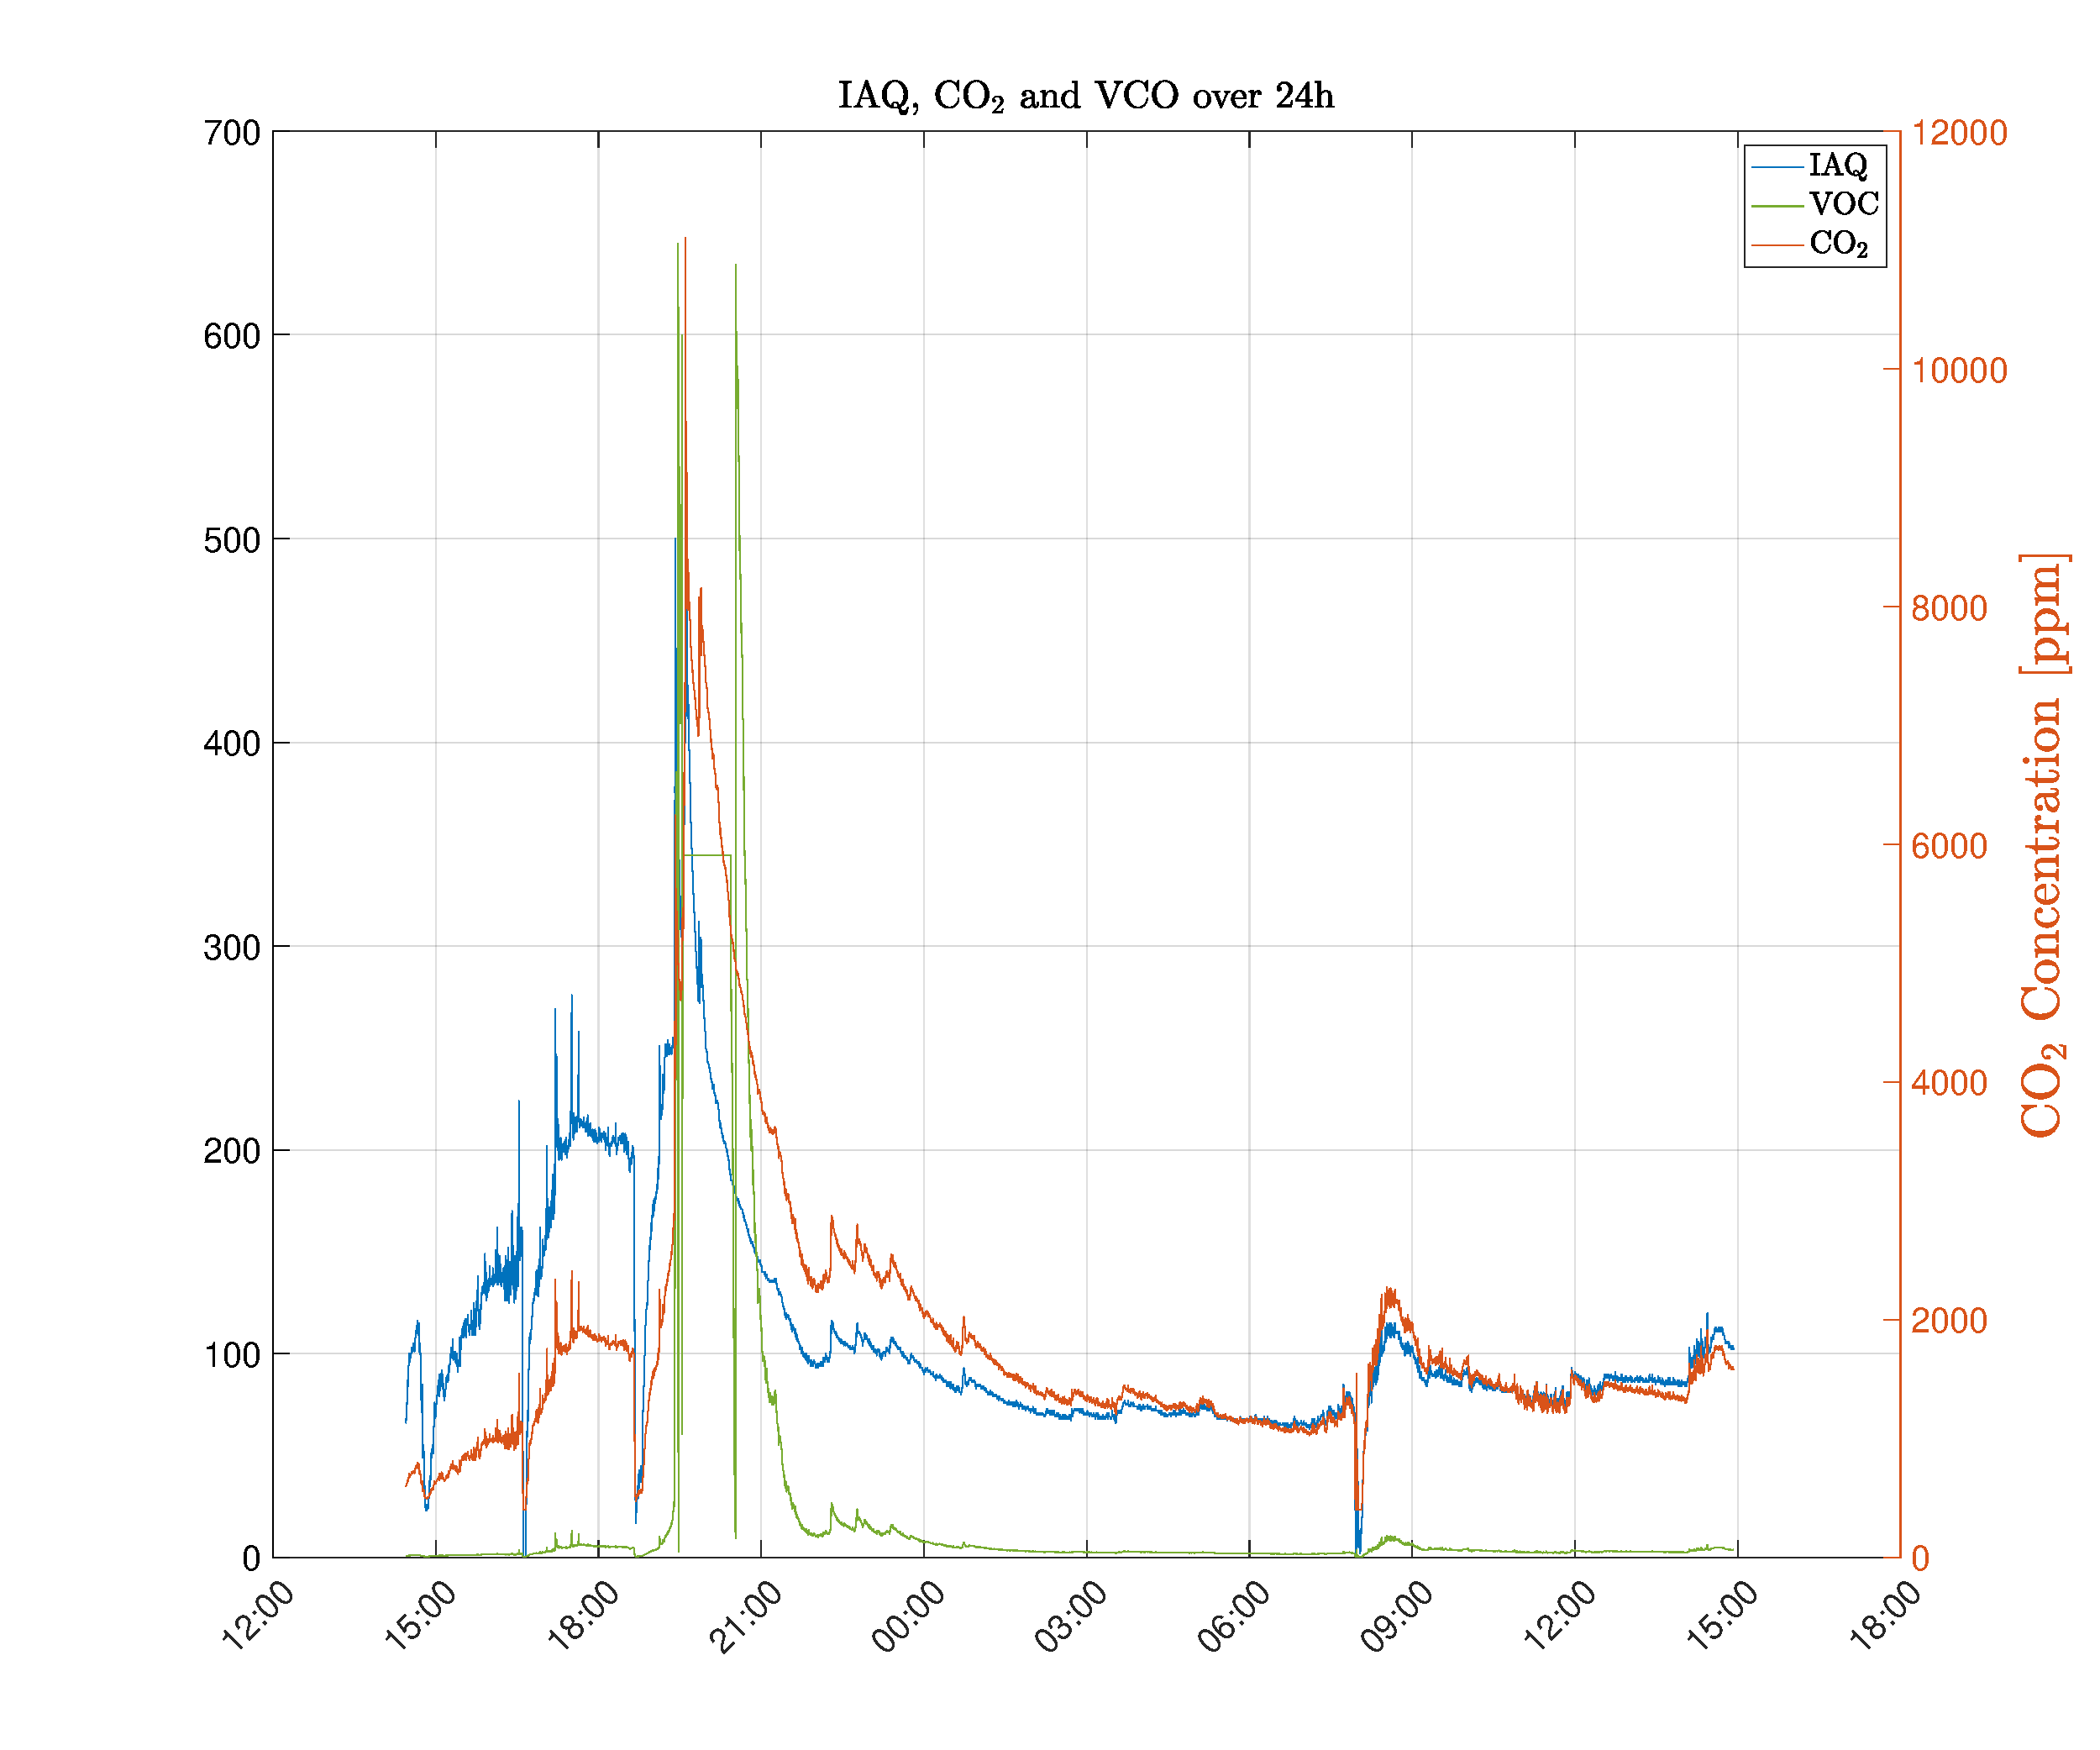
\includegraphics[width=.8\textwidth]{plots/plotCO2IAQVOC}
        \caption{$\mathrm{CO_2}$, IAQ and VOC over 24h.}
        \label{fig:iaqCO2VOC}
    \end{figure}

    We see that the IAQ seems realistic, and it basically follows the value of $\mathrm{CO_2}$ detection.
    \section{Summary}
    Experiments show that the gas sensor readings are stable even-though they present an offset in the temperature.
    The IAQ values are realistic.
    During the 24h measurements the events that happened are visible in the measurements.




% BibTeX or Biber would be better options, with just 2 reference the "raw" approach is fine for such a report
    \begin{thebibliography}{------}

        \bibitem[1]{labManual} J. Kieninger, S.\,J. Rupitsch, \textit{Sensors Lab Course}.
        University Freiburg.
        Winter term 2022/23.
        \bibitem[2]{BME688} \textit{BME688 Datasheet}, Bosch Sensortec, BST-BME688-DS000-01, rev. 1.1, July 2022.
        \bibitem[3]{Prill} Prill, Rich \textit{Why Measure Carbon Dioxide Inside Buildings?}.
        Washington State University Extension Energy Program.
        Available:https://www.energy.wsu.edu/documents/co2inbuildings.pdf. [Accessed: 18-Jan-2023]
        \bibitem[4]{EPA} \textit{What are volatile organic compounds (VOCs)?}, United States Environmental Protection Agency,
        Available: https://www.epa.gov/indoor-air-quality-iaq/what-are-volatile-organic-compounds-vocs. [Accessed: 18-Jan-2023]
        \bibitem[5]{EPA2} \textit{Volatile Organic Compounds' Impact on Indoor Air Quality}, United States Environmental Protection Agency,
        Available: https://www.epa.gov/indoor-air-quality-iaq/volatile-organic-compounds-impact-indoor-air-quality. [Accessed: 18-Jan-2023]
        \bibitem[6]{UST} \textit{Functional principle of Metal-oxide(MOX) gas sensor elements}. Umwelt Sensor Technik.
        https://www.umweltsensortechnik.de/en/gas-sensors/mox-gas-sensors-functional-principle.html. [Accessed: 18-Jan-2023]
        \bibitem[7]{Sensirion} https://sensirion.com/products/technology/. [Accessed: 19-Jan-2023]
    \end{thebibliography}


\end{document}
